\[\prod_{i \in I} X_i\ \text{到积空间}\ \prod_{x \in K} X_x'\]

是一个同胚。

这是初始拓扑的传递性的一个特殊情形（§ 2，第 3 目，命题 5；参见《集合论》，第四章，§ 2，第 4 目，判别准则 CST 13）。

通常我们借助典范映射把积空间 \(\prod_{i\in I}X_i\) 与 \(\prod_{x\in X}X_x'\) 等同起来。

推论. 设 \(\sigma\) 是集合 I 的一个置换。则映射 \((x_{i})\to (x_{\sigma(i)})\) 是

\[
\prod_ {i \in I} X _ {i} \quad onto \quad \prod_ {i \in I} X _ {\sigma (i)}.
\]

在命题 2 中取 \(\mathbf{K} = \mathbf{I}\) 及 \(\mathbf{J}_t = \{\sigma(t)\}\)（对每个 \(t \in I\)）。

命题 3. 设 X 是一个集合，\((\mathbf{Y}_{t})_{t\in I}\) 是拓扑空间的一个族，且对每个 \(t\in I\)，设 \(f_{t}\) 是 X 到 \(Y_{t}\) 中的一个映射。设 f 是映射 \(x\to(f_{t}(x))\)，把 X 映入 \(Y=\prod_{t\in I}Y_{t}\)，并设 G 是 X 上使诸映射 \(f_{t}\) 连续的最粗的拓扑。则 G 是 Y 上的积拓扑在 \(f(\mathbf{X})\) 上诱导的拓扑在 f 下的逆像。

这是初始拓扑的传递性的又一个特殊情形（§ 2，第 3 目，命题 5；参见《集合论》，第四章，§ 2，第 4 目，判别准则 CST 15）。

推论. 对每个 \(t \in I\)，设 \(A_{t}\) 是 \(Y_{t}\) 的一个子空间。则在 \(A = \prod_{t \in I} A_{t}\) 上由 \(\prod_{t \in I} Y_{t}\) 上的积拓扑诱导的拓扑是诸子空间 \(A_{t}\) 的拓扑之积。

设 \(j_{i}\) 是典范单射 \(A_{i} \to Y_{i}\)，并对诸映射 \(f_{i} = j_{i} \circ \operatorname{pr}_{i}\) 应用命题 3（参见《集合论》，第四章，§ 2，第 4 目，判别准则 GST 14）。

\subsection{开集的截面；闭集的截面；开集的投影。部分连续性}

命题 4. 设 \(\mathbf{X}_1, \mathbf{X}_2\) 是两个拓扑空间；则对每个 \(a_1 \in \mathbf{X}_1\)，映射 \(x_2 \to (a_1, x_2)\) 是 \(\mathbf{X}_2\) 映到 \(\{a_1\} \times \mathbf{X}_2\)（\(\mathbf{X}_1 \times \mathbf{X}_2\) 的子空间）上的一个同胚。

这是把第 1 目命题 1 的推论 1 应用于常值函数 \(x_{2} \rightarrow a_{1}\) 而得的一个特殊情形。

映射 \(x_{2} \to (a_{1}, x_{2})\) 是关于等价关系 \(\mathrm{pr}_{2}z = \mathrm{pr}_{2}z'\)（在 \(\mathbf{X}_{1} \times \mathbf{X}_{2}\) 中）的一个连续截面（§ 3，第 5 目）；因此 \(\mathbf{X}_{1} \times \mathbf{X}_{2}\) 按此等价关系的商空间同胚于 \(\mathbf{X}_{2}\)。

推论. 截面 \(\mathbf{A}(x_1)\)（开（相应地，闭）集 \(\mathbf{A}\)——积 \(\mathbf{X}_1 \times \mathbf{X}_2\) 的——在任意一点 \(x_1 \in \mathbf{X}_1\)（*）处的截面）在 \(\mathbf{X}_2\) 中是开（相应地，闭）集。

命题 5. 积 \(X_{1} \times X_{2}\) 的开集 U 到任一因子上的投影是开集。

例如，我们有 \(\mathrm{pr}_2\mathrm{U} = \bigcup_{x_1\in X_1}\mathrm{U}(x_1)\)，于是由命题 4 的推论及公理 \((\mathbf{O}_{\mathbf{I}})\) 即得该命题。

\pandocbounded{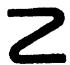
\includegraphics[keepaspectratio]{images/part001_fc188d82.jpg}}

注 1. \(\mathbf{X}_1 \times \mathbf{X}_2\) 的闭子集到一个因子上的投影未必是闭集。例如，在有理平面 \(\mathbf{Q}^2\) 中，方程为 \(x_1 x_2 = 1\) 的双曲线是闭集，但它的两个投影都等于 \(\mathbf{Q}\) 中点 0 的余集，而这不是闭集。

命题 6. 设 \(\mathbf{X}_1, \mathbf{X}_2, \mathbf{Y}\) 是三个拓扑空间，\(f\) 是积空间 \(\mathbf{X}_1 \times \mathbf{X}_2\) 到 \(\mathbf{Y}\) 中的一个映射。若 \(f\) 在点 \((a_1, a_2)\) 处连续，则部分映射 \(x_2 \to f(a_1, x_2)\)（\(\mathbf{X}_2\) 到 \(\mathbf{Y}\) 中的）在点 \(a_2\) 处连续。

因为这个映射是 \(f\) 与映射 \(x_{2} \to (a_{1}, x_{2})\) 的复合，故结论由命题 4 得出。

命题 6 常被表述为：两个变量的连续函数关于每个变量分别连续。

\pandocbounded{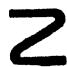
\includegraphics[keepaspectratio]{images/part001_31ca3096.jpg}}

注 2. 由映射 \(f: \mathbf{X}_{1} \times \mathbf{X}_{2} \to \mathbf{Y}\) 所确定的所有部分映射都连续，而 \(f\) 在 \(\mathbf{X}_{1} \times \mathbf{X}_{2}\) 上不连续，这是可能的（参见第九章，§ 5，习题 23）。* 例如，若 \(f\) 是实平面 \(\mathbb{R}^{2}\) 到 \(\mathbb{R}\) 中的映射，其定义为

\[
f (x, y) = x y / \left(x ^ {2} + y ^ {2}\right) \quad \text { if } \quad (x, y) \neq (0, 0)
\]

且 \(f(0, 0) = 0\)，则所有部分映射都连续；但 \(f\) 在 \((0, 0)\) 处不连续，因为 \(f(x, x) = 1/2\)（对 \(x \neq 0\)）。

若 \(g\) 是 \(\mathbf{X}_1\) 到 \(\mathbf{Y}\) 中的一个映射，在点 \(a_1\) 处连续，则映射 \((x_1, x_2) \to g(x_1)\)（\(\mathbf{X}_1 \times \mathbf{X}_1 \to \mathbf{Y}\)）在所有点 \((a_1, x_2)\) 处连续，因为它是 \(g\) 与到 \(\mathbf{X}_1\) 上的投影的复合。

本小节的结果容易推广到拓扑空间的任意积 \(\prod_{i\in I}X_i\)，只需注意到对 I 的任意分拆 (J, K)，这个积同胚于积 \(\left(\prod_{i\in J}X_i\right)\times\left(\prod_{i\in K}X_i\right)\)（第 1 目，命题 2）。

\subsection{积中的闭包}

命题 7. 在积空间 \(\prod_{i\in I}X_i\) 中，集合的积 \(\prod_{i\in I}A_i\) 的闭包与它们的闭包的积 \(\prod_{i\in I}\overline{A}_i\) 相同。

设 \(a = (a_{t})\) 属于 \(\prod_{i} A_{i}\) 的闭包；则对每个 \(x \in I\)，\(a_{x} = \text{pr}_{x} a\) 属于 \(A_{x}\) 的闭包，这是由于 \(\text{pr}_{x}\) 的连续性（\(\S 2\)，第 1 目，定理 1），因此 \(a \in \prod_{i} \overline{A}_{i}\)。反之，设 \(b = (b_{i}) \in \prod_{i} \overline{A}_{i}\)，并设 \(\prod_{i} V_{i}\) 是包含 \(b\) 的任一初等集；对每个 \(i \in I\)，\(V_{i}\) 包含一点 \(x_{i} \in A_{i}\)；于是 \(\prod_{i} V_{i}\) 包含点 \((x_{i}) \in \prod_{i} A_{i}\)，因此 \(b\) 属于 \(\prod A_{i}\) 的闭包。

推论. 非空集合的积 \(\prod_{i} A_{i}\) 在积空间 \(\prod_{i} X_{i}\) 中是闭集，当且仅当 \(A_{i}\) 在 \(X_{i}\) 中是闭集（对每个 \(i \in I\)）。

若 I 是有限集，则积 \(\prod_{i\in I}A_i\) 是开集，只要 \(A_i\) 在 \(X_i\) 中是开集（对每个 \(i\in I\)）；但当 I 是无限集时情况不再如此。

命题 8. 设 \(a = (a_{i})\) 是积空间 \(X = \prod_{i \in I} X_{i}\) 的任一点；则集合 \(D\)——由这样的点 \(x \in X\) 组成：\(\operatorname{pr}_{i} x = a_{i}\) 对除有限多个外的指标 \(i\) 成立——在 \(X\) 中稠密。

对每个 \(x \in \mathbf{X}\) 及每个初等集 \(V = \prod_{i \in I} U_i\)（包含 \(x\) 的），我们有 \(U_i = X_i\)，但指标 \(i\) 属于有限子集 \(J\)（\(I\) 的）者除外；若取 \(y_i = x_i\)（对 \(i \in J\)）、\(y_i = a_i\)（对 \(i \notin J\)），则显然有

\[
y = (y _ {i}) \in D \quad \text { and } \quad y \in V;
\]

由此即得结论。

\subsection{拓扑空间的逆极限}

设 I 是一个偏序（但不一定有向）集（*），其上的序关系记作 \(\alpha \leqslant \beta\)。对每个 \(\alpha \in I\)，设 \(X_{\alpha}\) 是一个拓扑空间，且对每一对 \((\alpha, \beta)\)（满足 \(\alpha \leqslant \beta\)），设 \(f_{\alpha\beta}\) 是 \(X_{\beta}\) 到 \(X_{\alpha}\) 中的一个映射。我们说 \((X_{\alpha}, f_{\alpha\beta})\) 是拓扑空间的一个逆系统，如果：1) \((X_{\alpha}, f_{\alpha\beta})\) 是集合的一个逆系统；2) \(f_{\alpha\beta}\) 是连续映射（每当 \(\alpha \leqslant \beta\)）。设 X 表示集合 \(\varprojlim X_{\alpha}\)，且对每个 \(\alpha \in I\)，设 \(f_{\alpha}\) 是典范映射 \(X \to X_{\alpha}\)；则 X 上使诸 \(f_{\alpha}\) 连续的最粗的拓扑称为（关于 \(f_{\alpha\beta}\) 的）诸 \(X_{\alpha}\) 的拓扑的逆极限，而赋有该拓扑的集合 X 称为拓扑空间的逆系统 \((X_{\alpha}, f_{\alpha\beta})\) 的逆极限。每当我们把 \(\varprojlim X_{\alpha}\) 作为拓扑空间来谈论时，总应理解成这个空间的拓扑是诸 \(X_{\alpha}\) 的拓扑的逆极限，除非另有明确说明。

集合 X 是积 \(\prod_{\alpha\in I}X_{\alpha}\) 的由满足下列条件的点 x 组成的子集：

\[
\operatorname{pr} _ {\alpha} (x) = f _ {\alpha \beta} (\operatorname{pr} _ {\beta} (x))\tag{I}
\]

每当 \(\alpha \leqslant \beta\)。由第 1 目命题 3 可知，诸 \(X_{\alpha}\) 的拓扑的逆极限与 \(X\) 上由积空间 \(\prod_{\alpha \in I} X_{\alpha}\) 的拓扑诱导的拓扑相同。若对每个 \(\alpha \in I\)，\(Y_{\alpha}\) 是 \(X_{\alpha}\) 的子空间，且诸 \(Y_{\alpha}\) 构成诸 \(X_{\alpha}\) 的子集的一个逆系统（《集合论》，第三章，§ 7，第 2 目），则显然拓扑空间 \(\varprojlim Y_{\alpha}\) 是 \(\varprojlim X_{\alpha}\) 的一个子空间。

设 \((\mathbf{X}_{\alpha}^{\prime}, f_{\alpha\beta}^{\prime})\) 是以同一集合 I 为指标集的拓扑空间的另一个逆系统，且对每个 \(\alpha \in I\)，设 \(u_{\alpha}: X_{\alpha} \to X_{\alpha}^{\prime}\) 是连续映射，使得 \((u_{\alpha})\) 是映射的一个逆系统；则 \(u = \varprojlim u_{\alpha}\) 是 \(X = \varprojlim X_{\alpha}\) 到 \(X^{\prime} = \varprojlim X_{\alpha}^{\prime}\) 中的一个连续映射。因为若 \(f_{\alpha}^{\prime}\) 是典范映射 \(X^{\prime} \to X_{\alpha}^{\prime}\)，我们有 \(f_{\alpha}^{\prime} \circ u = u_{\alpha} \circ f_{\alpha}\)，从而 \(f_{\alpha}^{\prime} \circ u\) 对每个 \(\alpha \in I\) 连续，于是断言由 § 2 第 3 目命题 4 得出。

最后，设 I 是有向集，并设 J 是 I 的一个共尾子集；设 Z 是拓扑空间的逆系统 \((\mathbf{X}_{\alpha}, f_{\alpha\beta})_{\alpha\in\mathbf{J}, \beta\in\mathbf{J}}\) 的逆极限。则典范双射 \(g: X \to Z\)（《集合论》，第三章，§ 7，第 2 目，命题 3）是一个同胚。因为我们有 \(\operatorname{pr}_{\lambda}(g(x)) = \operatorname{pr}_{\lambda}(x)\)（对每个 \(\lambda \in J\)）；故 g 连续（第 1 目，命题 1）；又若 h 是 g 的逆，则对每个 \(\alpha \in I\)，存在 \(\lambda \in J\) 使 \(\alpha \leqslant \lambda\)，从而 \(\operatorname{pr}_{\alpha}(h(z)) = f_{\alpha\lambda}(\operatorname{pr}_{\lambda}(z))\)；由于诸 \(f_{\alpha\lambda}\) 连续，这表明 h 连续（第 1 目，命题 1）。

命题 9. 设 I 是有向集，J 是 I 的一个共尾子集。设 \((\mathbf{X}_{\alpha}, f_{\alpha \beta})\) 是以 I 为指标集的拓扑空间的一个逆系统；设 \(\mathbf{X} = \varprojlim \mathbf{X}_{\alpha}\)，并设 \(f_{\alpha}: \mathbf{X} \to \mathbf{X}_{\alpha}\) 是典范映射。则由诸集合 \(\overline{f}_{\alpha}^{1}(\mathbf{U}_{\alpha})\) 组成的族（其中 \(\alpha\) 取遍 J，\(\mathbf{U}_{\alpha}\) 取遍基 \(\mathfrak{B}_{\alpha}\)——\(\mathbf{X}_{\alpha}\) 的拓扑的基，对每个 \(\alpha \in \mathbf{J}\)）是 \(\mathbf{X}\) 的拓扑的一个基。

由 § 2 第 3 目可知，形如 \(\overline{f}_{\alpha}^{1}(\mathbf{U}_{\alpha})\)（\(\alpha \in \mathbf{I}\)，\(\mathbf{U}_{\alpha}\) 是 \(\mathbf{X}_{\alpha}\) 中的开集）的集合的有限交组成 \(\mathbf{X}\) 的拓扑的一个基。若 \((\alpha_i)_{1 \leqslant i \leqslant n}\) 是 \(\mathbf{I}\) 的一个有限指标族，则存在 \(\gamma \in \mathbf{J}\)，使 \(\alpha_i \leqslant \gamma\)（对 \(1 \leqslant i \leqslant n\)）；从而 \(f_{\alpha_i} = f_{\alpha_i \gamma} \circ f_\gamma\)；若令

\[
\begin{array}{c} \mathrm{V} _ {\gamma} = \bigcap_ {i} \overline {{f}} _ {\alpha_ {i} \gamma} ^ {1} (\mathrm{U} _ {\alpha_ {i}}), \\ \overline {{f}} _ {\gamma} ^ {1} (\mathrm{V} _ {\gamma}) = \bigcap_ {i} \overline {{f}} _ {\alpha_ {i}} ^ {1} (\mathrm{U} _ {\alpha_ {i}}); \end{array}
\]

则我们有

而 \(V_{\gamma}\) 是开集，因而是属于 \(\mathfrak{B}_{\gamma}\) 的一些集合之并。由此即得结论。

推论. 设 A 是 X 的一个子集，且用 \(A_{\alpha}\) 表示 \(f_{\alpha}(A)\)（对每个 \(\alpha \in I\)）。则：

\begin{enumerate}
\def\labelenumi{(\roman{enumi})}
\item
  诸 \(\mathbf{A}_{\alpha}\)（相应地，诸 \(\overline{\mathbf{A}}_{\alpha}\)）构成诸 \(\mathbf{X}_{\alpha}\) 的子集的一个逆系统，且 \(\overline{\mathbf{A}} = \bigcap_{\alpha} \overline{f}_{\alpha}^{1}(\overline{\mathbf{A}}_{\alpha}) = \varprojlim \overline{\mathbf{A}}_{\alpha}\)。
\item
  若 A 在 X 中是闭集，则 \(\mathbf{A} = \varprojlim \mathbf{A}_{\alpha} = \varprojlim \overline{\mathbf{A}}_{\alpha}\)。
\end{enumerate}

(i) 的第一个断言由诸关系 \(f_{\alpha} = f_{\alpha \beta} \circ f_{\beta}\)（对 \(\alpha \leqslant \beta\)）及诸 \(f_{\alpha \beta}\) 的连续性得出（§ 2，第 1 目，定理 1）。用 \(A'\) 表示

\[
\bigcap_ {\alpha} \overline {{f}} _ {\alpha} ^ {1} (\overline {{\mathrm{A}}} _ {\alpha});
\]

则显然 \(\mathbf{A}'\) 是闭集且包含 \(\mathbf{A}\)，从而 \(\overline{\mathbf{A}} \subset \mathbf{A}'\)。反之，设 \(x \in \mathbf{A}'\)；我们必须证明 \(x\) 属于 \(\mathbf{A}\) 的闭包。凭借命题 9，只须证明 \(x\) 的每个形如 \(\overline{f}_{\alpha}^{1}(\mathrm{U}_{\alpha})\) 的邻域（其中 \(\alpha \in \mathbf{I}\)，\(\mathbf{U}_{\alpha}\) 是 \(\mathbf{X}_{\alpha}\) 中的开集）都与 \(\mathbf{A}\) 相交。而按假设，\(f_{\alpha}(x) \in \mathbf{U}_{\alpha}\)，又因 \(f_{\alpha}(x) \in \overline{\mathbf{A}}_{\alpha}\)，我们有 \(\mathbf{U}_{\alpha} \cap \mathbf{A}_{\alpha} \neq \emptyset\)，这就意味着 \(\mathbf{A} \cap \overline{f}_{\alpha}^{1}(\mathbf{U}_{\alpha})\) 非空。

为建立 (ii)，只须注意，对 A 不加任何限制时，我们有 \(A \subset \varprojlim A_{\alpha} \subset \varprojlim \overline{A}_{\alpha}\)；而若 A 是闭集，则由 (i)

\[
\mathrm{A} = \varprojlim \overline {{\mathrm{A}}} _ {\alpha}
\]

便得 (ii)。

例. 设 I 是有向集，\((\mathbf{X}_{\alpha})_{\alpha \in I}\) 是集合 Y 的子集的一个族，使得 \(\mathbf{X}_{\alpha} \supset \mathbf{X}_{\beta}\)（每当 \(\alpha \leqslant \beta\)）。对每个 \(\alpha \in I\)，设 \(\mathfrak{G}_{\alpha}\) 是 \(\mathbf{X}_{\alpha}\) 上的一个拓扑，使得 \(\mathfrak{G}_{\beta}\) 都细于 \(\mathbf{X}_{\beta}\) 上由 \(\mathfrak{G}_{\alpha}\) 诱导的拓扑（每当 \(\alpha \leqslant \beta\)）。若取 \(f_{\alpha \beta}\) 为典范单射 \(\mathbf{X}_{\beta} \to \mathbf{X}_{\alpha}\)（对 \(\alpha \leqslant \beta\)），则 \(\varprojlim \mathbf{X}_{\alpha}\) 可以典范地等同于诸 \(\mathbf{X}_{\alpha}\) 的交 X，赋以诸拓扑之上确界（§ 2，第 3 目，例 2）——这些拓扑由诸 \(\mathfrak{G}_{\alpha}\) 在 X 上诱导。

\section{开映射与闭映射}

\subsection{开映射与闭映射}

定义 1. 设 X、X' 是两个拓扑空间。映射 f: X → X' 称为开（相应地，闭）映射，如果 X 的每个开（相应地，闭）集在 f 下的像在 X' 中是开（相应地，闭）集。

特别地，此时 \(f(\mathbf{X})\) 是 \(X'\) 的开（相应地，闭）子集。

例。1) 设 A 是拓扑空间 X 的一个子空间。则典范单射 \(j: \mathbf{A} \to \mathbf{X}\) 是开（相应地，闭）映射，当且仅当 A 在 X 中是开（相应地，闭）集（\(\S\) 3，第 1 目）。

\begin{enumerate}
\def\labelenumi{\arabic{enumi})}
\setcounter{enumi}{1}
\item
  为使双射 \(f\)（从拓扑空间 \(\mathbf{X}\) 到拓扑空间 \(\mathbf{X}'\) 上的）是一个同胚，必须且只需 \(f\) 连续且开，或连续且闭。
\item
  设 \(f\) 是集合 \(X\) 到拓扑空间 \(X'\) 上的一个满射；若给 \(X\) 赋以在 \(f\) 之下 \(X'\) 的拓扑的逆像这一拓扑（§ 2，第 3 目，例 1），则 \(f\) 连续、开且闭。
\item
  在积空间
\end{enumerate}

\[
\mathbf {X} = \prod_ {i \in \mathbf {I}} \mathbf {X} _ {i},
\]

中，每个投影 \(\mathbf{pr}_{t}:\mathbf{X}\to\mathbf{X}_{t}\) 都是连续的开映射，但未必是闭映射（§ 4，第 2 目，命题 5）。

* 5) 在 C 的开子集 A 上的全纯函数是 A 到 C 中的一个开映射。*

\begin{enumerate}
\def\labelenumi{\arabic{enumi})}
\setcounter{enumi}{5}
\tightlist
\item
  设 X、X' 是两个拓扑空间，f 是 X 到 X' 上的一个连续但非双连续的双射。则逆双射 g: \(X' \rightarrow X\) 是 \(X'\) 到 X 上的一个既开又闭的映射，但不连续。
\end{enumerate}

命题 1. 设 X、X'、X'' 是三个拓扑空间，并设 f: X → X'、g : X' → X'' 是两个映射。则：

\begin{enumerate}
\def\labelenumi{\alph{enumi})}
\item
  若 \(f\) 与 \(g\) 是开（相应地，闭）映射，则 \(g \circ f\) 亦然。
\item
  若 \(g \circ f\) 是开（相应地，闭）映射且 \(f\) 连续并满，则 \(g\) 是开（相应地，闭）映射。
\item
  若 \(g \circ f\) 是开（相应地，闭）映射且 \(g\) 连续并单，则 \(f\) 是开（相应地，闭）映射。
\end{enumerate}

a) 由定义 1 立即得出。为证 b)，只须注意，每个开（相应地，闭）子集 \(\mathbf{A}'\)（\(\mathbf{X}'\) 的）都可写成 \(f(\mathbf{A})\)，其中 \(\mathbf{A} = \overline{f}^{1}(\mathbf{A}')\) 在 \(\mathbf{X}\) 中是开（相应地，闭）集（\(\S 2\)，第 1 目，定理 1）；从而 \(g(\mathbf{A}') = g(f(\mathbf{A}))\) 在 \(\mathbf{X}''\) 中是开（相应地，闭）集。最后，为证 c)，我们注意，\(f(\mathbf{A}) = \overline{g}^{1}(g(f(\mathbf{A}))\) 对每个子集 \(\mathbf{A}\)（\(\mathbf{X}\) 的）成立；按假设，若 \(\mathbf{A}\) 在 \(\mathbf{X}\) 中是开（相应地，闭）集，则 \(g(f(\mathbf{A}))\) 在 \(\mathbf{X}''\) 中是开（相应地，闭）集，从而 \(f(\mathbf{A})\) 在 \(\mathbf{X}'\) 中是开（相应地，闭）集（\(\S 2\)，第 1 目，定理 1）。

命题 2. 设 X、Y 是两个拓扑空间，f 是 X 到 Y 中的一个映射。对 Y 的每个子集 T，用 \(f_{T}\) 表示 \(\overline{f}^{1}(T)\) 到 T 中的、在 \(\overline{f}^{1}(T)\) 上与 f 一致的映射。

\begin{enumerate}
\def\labelenumi{\alph{enumi})}
\item
  若 \(f\) 是开（相应地，闭）映射，则 \(f_{\mathbf{T}}\) 是开（相应地，闭）映射。
\item
  设 \((\mathbf{T}(\iota))_{\iota \in \mathbf{I}}\) 是 Y 的子集的一个族，其诸内部覆盖 Y，或者它是 Y 的一个局部有限闭覆盖；若所有 \(f_{\mathbf{T}(\iota)}\) 都是开（相应地，闭）映射，则 \(f\) 是开（相应地，闭）映射。
\item
  若 A 是 \(\overline{f}^{1}(\mathbf{T})\) 的开（相应地，闭）子集，则存在 X 的开（相应地，闭）子集 B，使 \(\mathbf{A} = \mathbf{B} \cap \overline{f}^{1}(\mathbf{T})\)，从而 \(f_{\mathbf{T}}(\mathbf{A}) = f(\mathbf{B}) \cap \mathbf{T}\)；按假设，\(f(\mathbf{B})\) 是开（相应地，闭）集，于是 \(f_{\mathbf{T}}(\mathbf{A})\) 在 \(\mathbf{T}\) 中是开（相应地，闭）集。
\item
  设 B 是 X 的开（相应地，闭）子集，并用 \(B_{i}\) 表示 \(\mathbf{B} \cap \overline{f}^{1}(\mathrm{T}(i))\)；则 \(f(\mathbf{B}) \cap \mathrm{T}(i) = f_{\mathbf{T}(i)}(\mathbf{B}_{i})\)。由于按假设 \(f_{\mathbf{T}(i)}(\mathbf{B}_{i})\) 在 \(\mathrm{T}(i)\) 中是开（相应地，闭）集，故由 § 3 第 1 目命题 3，\(f(\mathbf{B})\) 在 Y 中是开（相应地，闭）集。
\end{enumerate}

推论. 设 \((\mathbf{T}(\iota))_{\iota \in \mathbf{I}}\) 是 Y 的子集的一个族，其诸内部覆盖 Y，或者它是 Y 的一个局部有限闭覆盖。若 \(f: \mathbf{X} \to \mathbf{Y}\) 连续，且每个 \(f_{\mathbf{T}(\iota)}\) 都是 \(\overline{f}^1 (\mathbf{T}(\iota))\) 到 \(\mathbf{T}(\iota)\) 上的一个同胚，则 \(f\) 是 \(\mathbf{X}\) 到 \(\mathbf{Y}\) 上的一个同胚。

因为 \(f\) 显然是双射，且凭借命题 2 是开映射。

\subsection{开等价关系与闭等价关系}

定义 2. 拓扑空间 X 上的等价关系 R 称为开（相应地，闭）的，如果 X 到 X/R 上的典范映射是开（相应地，闭）映射。

这等价于说，X 的每个开（相应地，闭）子集关于 R 的饱和化在 X 中是开（相应地，闭）集（§ 3，第 4 目）。

例。1) 设 X 是拓扑空间，\(\Gamma\) 是 X 到自身的一些同胚所成的一个群，并设 R 是等价关系

\[
" \text { there   exists } \sigma \in \Gamma \text { such   that } y = \sigma (x)"
\]

（x 与 y 之间）（于是 R 是以 \(\Gamma\) 在 X 中的轨道为类的那个等价关系。关系 R 是开的，因为 X 的子集 A 关于 R 的饱和化是开集，诸 \(\sigma(\mathbf{A})\) 也是开集，从而它们的并也是开集。

* 在实直线 R 上，等价关系 \(x \equiv y \pmod{1}\) 是开的，因为它如上所述由平移群

\[
x \rightarrow x + n \quad (n \in \mathbf {Z})
\]

导出（见第三章，§ 2，第 4 目）。*

\begin{enumerate}
\def\labelenumi{\arabic{enumi})}
\setcounter{enumi}{1}
\tightlist
\item
  设 X 是子空间族 \((\mathbf{X}_{t})\) 的和，并设 X/R 是把诸 \(X_{t}\) 沿开子集 \(A_{tx}\) 借助双射 \(h_{xt}\) 粘合起来所得的空间（§ 2，第 5 目）；并设 \(h_{xt}\) 是 \(A_{tx}\) 到 \(A_{xt}\) 上的一个同胚（对每一对指标 \((t, x)\)）。
\end{enumerate}

则关系 R 是开的。因为若 U 在 X 中是开集，则 U 的饱和化是诸 \(h_{xt}(\mathbf{U} \cap \mathbf{A}_{\mathbf{tx}})\) 之并；由于 \(U \cap A_{tx}\) 在 \(A_{tx}\) 中是开集，故 \(h_{xt}(\mathbf{U} \cap \mathbf{A}_{\mathbf{tx}})\) 在 \(A_{xt}\) 中从而在 X 中是开集。

\begin{enumerate}
\def\labelenumi{\arabic{enumi})}
\setcounter{enumi}{2}
\tightlist
\item
  沿用例 2 的记号，现在设诸 \(\mathbf{A}_{\mathrm{tx}}\) 是闭集且诸 \(h_{xt}\) 是同胚；再设对每个指标 \(t\)，只有有限多个指标 \(x\) 使 \(\mathbf{A}_{\mathrm{tx}} \neq \emptyset\)（亦即每个 \(\mathbf{X}_t\) 只与有限多个 \(\mathbf{X}_x\) 相“粘”）。则关系 R 是闭的。因为若 F 是 X 的任一闭子集，则 F 的饱和化是诸集合 \(h_{xt}(\mathbf{F} \cap \mathbf{A}_{\mathrm{tx}}) \subset \mathbf{A}_{xt}\) 之并；所作的假定蕴含这一族是局部有限的，且 \(h_{xt}(\mathbf{F} \cap \mathbf{A}_{\mathrm{tx}})\) 在 \(\mathbf{A}_{xt}\) 中从而在 X 中是闭集。于是结论由 § 2 第 5 目命题 4 得出。
\end{enumerate}

命题 3. 设 X、Y 是两个拓扑空间，设 \(f: \mathbf{X} \to \mathbf{Y}\) 是连续映射，设 R 是 X 上的等价关系 \(f(x) = f(y)\)，并设 \(\mathbf{X} \xrightarrow{p} \mathbf{X}/\mathbf{R} \xrightarrow{h} f(\mathbf{X}) \xrightarrow{i} \mathbf{Y}\) 是 \(f\) 的典范分解。则下列三个命题等价：

\begin{enumerate}
\def\labelenumi{\alph{enumi})}
\item
  \(f\) 是开映射。
\item
  三个映射 \(p, h, i\) 都是开映射。
\item
  等价关系 R 是开的，h 是同胚，且 \(f(\mathbf{X})\) 是 Y 的开子集。
\end{enumerate}

还有，若把前面命题中的“开”处处换为“闭”，该命题仍成立。

由于单射 \(i\) 连续，由第 1 目命题 1c) 可知，若 \(f\) 是开映射，则 \(h \circ p\) 亦然；由于 \(p\) 满且连续，命题 1b) 表明 \(h\) 是开映射；\(h\) 无论如何是连续双射；于是 \(h\) 是同胚，从而由第 1 目命题 1a)，\(p = \overline{h}^1 \circ (h \circ p)\) 是开映射。又有{[}第 1 目，命题 1b){]}，\(i \circ h\) 是开映射；故{[}第 1 目，命题 1a){]}，\(i = (i \circ h) \circ \overline{h}^1\) 亦然。这就证明了 a) 蕴含 b)。反之，第 1 目命题 1a) 表明 b) 蕴含 a)。最后，b) 与 c) 的等价性由定义立即得出。

闭映射情形的证明，作适当改动后是类似的。

命题 4. 设 R 是拓扑空间 X 上的开（相应地，闭）等价关系，f 是典范映射 X → X/R。设 A 是 X 的一个子集，且下列两个条件之一成立：a) A 在 X 中是开（相应地，闭）集。

\begin{enumerate}
\def\labelenumi{\alph{enumi})}
\setcounter{enumi}{1}
\tightlist
\item
  A 关于 R 是饱和的。
\end{enumerate}

则在 A 上诱导的关系 \(R_{A}\) 是开（相应地，闭）的，且 \(A/R_{A}\) 到 \(f(A)\) 上的典范映射是同胚。

考虑 § 3 第 6 目的交换图 (1)，它给出 \(f \circ j\) 的典范分解。在条件 a) 下，\(j\) 是开（相应地，闭）映射，而按假设 \(f\) 亦然；故 \(f \circ j\) 是开（相应地，闭）映射{[}第 1 目，命题 1 a){]}，结论由命题 3 得出。在条件 b) 下，我们有

\[
\mathbf {A} = \overline {{{f}}} ^ {1} (f (\mathbf {A})),
\]

且 \(h \circ \varphi\) 是 A 到 \(f(A)\) 中的、在 A 上与 \(f\) 一致的映射；凭借第 1 目命题 2 a)，\(h \circ \varphi\) 是开（相应地，闭）映射，而把命题 3 应用于 \(h \circ \varphi\)，又得出结论。

\subsection{开映射特有的性质}

命题 5. 设 X、Y 是两个拓扑空间，f 是 X 到 Y 中的一个映射，B 是 X 的拓扑的一个基。则下列命题等价：

\begin{enumerate}
\def\labelenumi{\alph{enumi})}
\item
  \(f\) 是开映射。
\item
  对每个 \(\mathbf{U} \in \mathfrak{B}\)，\(f(\mathbf{U})\) 在 \(\mathbf{Y}\) 中是开集。
\item
  对每个 \(x \in \mathbf{X}\) 及每个邻域 \(\mathbf{V}\)（\(x\) 的，\(\mathbf{X}\) 中的），\(f(\mathbf{V})\) 都是 \(f(x)\) 在 \(\mathbf{Y}\) 中的一个邻域。
\end{enumerate}

a) 与 b) 的等价性由定义及 \((\mathrm{O}_{\mathrm{I}})\) 立即得出；a) 与 c) 的等价性是 § 1 第 2 目命题 1 的推论。

命题 6. 设 R 是拓扑空间 X 上的一个等价关系；则下列三个条件等价：

\begin{enumerate}
\def\labelenumi{\alph{enumi})}
\item
  关系 \(\mathbf{R}\) 是开的。
\item
  每个关于 R 饱和的子集，其内部关于 R 是饱和的。
\item
  每个关于 R 饱和的子集，其闭包关于 R 是饱和的。
\end{enumerate}

取余集（§ 1，第 6 目，公式 (2)）可见 b) 与 c) 等价。我们来证 b) 蕴含 a)：设条件 b) 成立，并设 U 是 X 的开子集，V 是它关于 R 的饱和化；则 \(\dot{V} \supset U\)，又因按假设 \(\dot{V}\) 是饱和的，故 \(\dot{V} = V\)，从而 U 的饱和化是开集。反之，设条件 a) 成立，并设 A 是一个饱和集；若 B 是 \(\mathring{A}\) 的饱和化，则 \(\mathring{A} \subset B \subset A\)，又因按假设 B 是开集，故 \(B = \mathring{A}\)。

命题 7. 设 R 是拓扑空间 X 上的开等价关系，并设 \(\varphi: \mathbf{X} \to \mathbf{X}/\mathbf{R}\) 是典范映射。若 A 是 X 的任一关于 R 饱和的子集，则 \(\varphi(\mathbf{A})\) 在 X/R 中的闭包（相应地，内部）是 \(\varphi(\overline{\mathbf{A}})\)（相应地，\(\varphi(\mathring{\mathbf{A}})\)）。

该命题的两个断言中的每一个都可由另一个通过取余集并利用 § 1 第 6 目公式 (2) 及下述事实导出：若 B 是 X 的饱和子集，则 \(\varphi(\complement B) = \complement \varphi(B)\)。凭借命题 6，\(\overline{A}\) 是饱和的；从而 \(\varphi(\overline{A})\) 在 \(X/R\) 中是闭集，又因 \(A \subset \overline{A}\)，我们有 \(\overline{\varphi(A)} \subset \varphi(\overline{A})\)，从而 \(\varphi(A) \subset \varphi(\overline{A})\)。但由 \(\varphi\) 连续，\(\varphi(\overline{A}) \subset \overline{\varphi(A)}\)（\(\S 2\)，第 1 目，定理 1），由此即得结论。

命题 8. 设 \((\mathbf{X}_t)_{t \in \mathbf{I}}\)、\((\mathbf{Y}_t)_{t \in \mathbf{I}}\) 是以同一集合 I 为指标集的两个拓扑空间族。对每个 \(t \in \mathbf{I}\)，设 \(f_t\) 是 \(\mathbf{X}_t\) 到 \(\mathbf{Y}_t\) 中的一个开映射，并设除去有限多个指标外 \(f_t\) 都是满射。则积映射 \(f: (x_t) \to (f_t(x_t))\)（\(\prod_{t \in \mathbf{I}} \mathbf{X}_t\) 到 \(\prod_{t \in \mathbf{I}} \mathbf{Y}_t\) 中的）是开映射。

凭借命题 5，我们只须证明 \(f\) 的任意初等集 \(\prod_{t \in I} A_t\)（\(\prod_{t \in I} X_t\) 中的）的像在 \(\prod_{t \in I} Y_t\) 中是开集。而这个像是 \(\prod_{t \in I} f_t(A_t)\)，且诸假设蕴含：\(f_t(A_t)\) 在 \(Y_t\) 中是开集（对每个 \(t \in I\)），且除去有限多个指标外 \(f_t(A_t) = Y_t\)；由此即得结论。

推论. 设 \((\mathbf{X}_t)_{t \in I}\) 是拓扑空间的一个族，且对每个 \(t \in I\)，设 \(\mathbf{R}_t\) 是 \(\mathbf{X}_t\) 上的一个等价关系，并设 \(f_t\) 是典范映射 \(\mathbf{X}_t \to \mathbf{X}_t / \mathbf{R}_t\)。设 \(\mathbf{R}\) 是 \(\mathbf{X} = \prod_{t \in I} \mathbf{X}_t\) 中的等价关系“对每个 \(t \in I\)，\(\operatorname{pr}_t(x) = \operatorname{pr}_t(y) (\bmod \mathbf{R}_t)"\)

（\(x\) 与 \(y\) 之间），并设 \(f\) 是积映射 \((x_{t}) \to (f_{t}(x_{t}))\)（\(X\) 到 \(\prod_{t \in I} (X_{t}/R_{t})\) 中的）。若诸关系 \(R_{t}\) 都是开的，则关系 \(R\) 是开的，且与 \(f\) 相伴的双射是 \(X/R\) 到 \(\prod_{t \in I} (X_{t}/R_{t})\) 上的一个同胚。

R 是关系 \(f(x)=f(y)\)。由于由上面的命题 8 及 § 4 第 1 目命题 1 的推论 1，f 连续且开，故结论由第 2 目命题 3 得出。

特别地，若 R（相应地，S）是拓扑空间 X（相应地，Y）上的开等价关系，则

\[
(\mathbf {X} \times \mathbf {Y}) / (\mathbf {R} \times \mathbf {S}) \quad \text { onto } \quad (\mathbf {X} / \mathbf {R}) \times (\mathbf {Y} / \mathbf {S})
\]

\pandocbounded{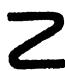
\includegraphics[keepaspectratio]{images/part001_bebaa45c.jpg}}

的典范双射是一个同胚。若不假定 R 与 S 都是开的，则这个双射连续但未必是同胚，即使关系 R、S 之一是相等关系（习题 6）亦然。

\subsection{闭映射特有的性质}

命题 9. 设 X、X' 是两个拓扑空间。映射 \(f: \mathbf{X} \to \mathbf{X}'\) 连续且闭的充分必要条件是：对 X 的每个子集 A，\(f(\overline{\mathbf{A}}) = \overline{f(\mathbf{A})}\)。

该条件是充分的，因为它显然蕴含 \(f\) 是闭映射，且由 § 2 第 1 目定理 1，它也蕴含 \(f\) 连续。反之，若 \(f\) 连续且闭，则由 § 2 第 1 目定理 1，我们有 \(f(\mathbf{A}) \subset f(\overline{\mathbf{A}}) \subset \overline{f(\mathbf{A})}\)；又按假设 \(f(\overline{\mathbf{A}})\) 在 \(\mathbf{X}'\) 中是闭集；从而 \(f(\overline{\mathbf{A}}) = \overline{f(\mathbf{A})}\)。

命题 10. 设 R 是拓扑空间 X 上的一个等价关系。则 R 是闭的，当且仅当模 R 的每个等价类 M 都具有由关于 R 饱和的邻域组成的一个基本邻域系。

设 R 是闭的，并设 U 是 M 的任一开邻域；由于 \(F = \complement U\) 在 X 中是闭集，F 关于 R 的饱和化 S 在 X 中是闭集。由于 M 关于 R 是饱和的，我们有 \(M \cap S = \varnothing\)，从而 \(V = \complement S\) 是 M 的一个开邻域，它关于 R 饱和且含于 U。

为证其逆，设 F 是 X 的任一闭子集。设 T 是 F 关于 R 的饱和化，设 x 是 \(\complement T\) 的一点，并设 M 是 x 的等价类；则 \(M \cap T = \varnothing\)，从而更有 \(M \cap F = \varnothing\)，于是 U = \(\complement F\) 是 M 的一个邻域。因此存在 M 的一个邻域 \(V \subset U\)，使 V 关于 R 饱和；V 不与 F 相交，故不与 T 相交，从而 \(\complement T\) 是 M 的、因而是 x 的一个邻域。这表明 \(\complement T\) 是开集（§ 1，第 2 目，命题 1），亦即 T 是闭集。

注. 命题 10 蕴含以下事实：若 R 是闭的，且用 \(\varphi\) 表示典范映射 \(X \to X/R\)，则对每个 \(x \in X\) 以及 \(x\) 的等价类在 X 中的每个邻域 U，\(\varphi(U)\) 都是 \(\varphi(x)\) 在 X/R 中的一个邻域。应当仔细注意，这一断言决不蕴含：对 \(x\) 的每个邻域 V，\(\varphi(V)\) 都是 \(\varphi(x)\) 的邻域；换言之（第 3 目，命题 5），闭等价关系未必是开的（习题 2）。反过来，开等价关系也未必是闭的（第 1 目，例 4）；

\pandocbounded{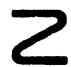
\includegraphics[keepaspectratio]{images/part001_bfecd507.jpg}}

因为若 U 是某个等价类 M 在 X 中的一个邻域，则对每个 \(x \in M\) 以及 x 的每个邻域 \(V \subset U\)，V 的饱和化固然是 M 在 X 中的一个邻域，但这个邻域未必含于 U。

最后，存在除相等关系之外既开又闭的等价关系（习题 3），也存在既不开又不闭的等价关系（\(§\ 8\)，习题 10）。

\section{滤子}

\subsection{滤子的定义}

定义 1. 集合 X 上的滤子是 X 的子集所成的一个集合 F，它具有下列性质：

（F \(_{I}\)）X 的每个包含 F 中某个集合的子集都属于 F。

\((\mathbf{F}_{\mathrm{II}})\) \(\mathfrak{F}\) 的集合的每个有限交都属于 \(\mathfrak{F}\)。

\((\mathbf{F}_{\mathrm{III}})\) 空集不属于 \(\mathfrak{F}\)。

由 \((\mathbf{F}_{\mathbf{II}})\) 与 \((\mathbf{F}_{\mathbf{III}})\) 可知，F 的集合的每个有限交都非空。

X 上的滤子 \(\mathfrak{F}\) 在 X 上定义了一个结构，其公理为 \((\mathrm{F_I})\)、\((\mathrm{F_{II}})\) 与 \((\mathrm{F_{III}})\)；这个结构称为滤集结构，而赋以该结构的集合 X 称为被 \(\mathfrak{F}\) 滤化的集合。

公理 \((\mathbf{F}_{\mathrm{II}})\) 等价于下列两条公理的合取：\((\mathbf{F}_{\mathrm{II}a})\) F 中两个集合的交属于 F。

\((\mathbf{F}_{\mathrm{II}b})\) X 属于 \(\mathfrak{F}\)。

公理 \((\mathbf{F}_{\mathbf{II}\ \mathbf{b}})\) 与 \((\mathbf{F}_{\mathbf{III}})\) 表明空集上不存在滤子。

为使满足 \((\mathbf{F}_{\mathbf{I}})\) 的子集族也满足 \((\mathbf{F}_{\mathbf{II}\mathbf{b}})\)，必须且只需它非空。满足 \((\mathbf{F}_{\mathbf{I}})\) 的子集族也满足 \((\mathbf{F}_{\mathbf{III}})\)，当且仅当它异于 \(\mathfrak{P}(\mathbf{X})\)。

滤子的例子. 1) 若 \(\mathbf{X} \neq \emptyset\)，则仅由 \(\mathbf{X}\) 组成的子集族是 \(\mathbf{X}\) 上的一个滤子。更一般地，\(\mathbf{X}\) 中包含给定非空子集 \(\mathbf{A}\)（\(\mathbf{X}\) 的）的所有子集所成之集是 \(\mathbf{X}\) 上的一个滤子。

\begin{enumerate}
\def\labelenumi{\arabic{enumi})}
\setcounter{enumi}{1}
\item
  在拓扑空间 X 中，X 的任一非空子集 A 的所有邻域所成之集（特别地，X 中一点的所有邻域所成之集）是一个滤子，称为 A 的邻域滤子。
\item
  若 X 是无限集，则 X 的有限子集的余集组成一个滤子的元素。由 \(\geqslant0\) 的整数组成的集 N 的有限子集的余集所成的滤子称为 Fréchet 滤子。
\end{enumerate}

\subsection{滤子的比较}

定义 2. 给定同一集合 X 上的两个滤子 \(\mathfrak{F}\)、\(\mathfrak{F}'\)，称 \(\mathfrak{F}'\) 细于 \(\mathfrak{F}\)，或称 \(\mathfrak{F}\) 粗于 \(\mathfrak{F}'\)，如果 \(\mathfrak{F} \subset \mathfrak{F}'\)。若还有 \(\mathfrak{F} \neq \mathfrak{F}'\)，则称 \(\mathfrak{F}'\) 严格细于 \(\mathfrak{F}\)，或称 \(\mathfrak{F}\) 严格粗于 \(\mathfrak{F}'\)。

若两个滤子中一个细于另一个，则称这两个滤子可比较。X 上所有滤子所成之集按关系“F 粗于 F”排序；这个关系是由 \(\mathfrak{P}(\mathfrak{P}(\mathbf{X}))\) 中的包含关系诱导的。

设 \((\mathfrak{F}_t)_{\iota \in I}\) 是集合 \(X\) 上滤子的任一非空族（因而 X 必非空）；则集合

\[
\mathfrak {F} = \bigcap_ {i \in I} \mathfrak {F} _ {i}
\]

满足公理 \((\mathbf{F}_{\mathbf{I}})\)、\((\mathbf{F}_{\mathbf{II}})\) 与 \((\mathbf{F}_{\mathbf{III}})\)，从而是一个滤子；F 称为滤子族 \((\mathfrak{F}_{i})_{i\in\mathbf{I}}\) 的交，并且显然是 X 上所有滤子之有序集中诸 \(F_{i}\) 所成之集的下确界。

由单独一个集合 X 组成的滤子是 X 上所有滤子之有序集的最小元。我们将在第 4 目看到，若 X 的元素多于一个，则 X 上所有滤子所成之集没有最大元。

给定集合 X 的一个子集族 \(\mathfrak{G}\)，我们来考察 X 上是否存在包含 \(\mathfrak{G}\) 的滤子。若这样的滤子存在，则由 \((\mathrm{F}_{\mathrm{II}})\)，它也包含集 \(\mathfrak{G}'\)（\(\mathfrak{G}\) 中集合的有限交所成之集，包括 X，即 \(\mathfrak{G}\) 的空子集之交）；因此这样的滤子存在的一个必要条件是 X 的空子集不属于 \(\mathfrak{G}'\)。这个条件也是充分的，因为由 \((\mathrm{F}_{\mathrm{I}})\)，任何包含 \(\mathfrak{G}'\) 的滤子也包含集 \(\mathfrak{G}''\)（X 中包含 \(\mathfrak{G}'\) 中某个集合的子集所成之集）。而 \(\mathfrak{G}''\) 显然满足 \((\mathrm{F}_{\mathrm{I}})\)；它满足 \((\mathrm{F}_{\mathrm{II}})\)（由 \(\mathfrak{G}'\) 的定义）；最后，它满足 \((\mathrm{F}_{\mathrm{III}})\)，因为 X 的空子集不属于 \(\mathfrak{G}'\)。于是 \(\mathfrak{G}''\) 是包含 \(\mathfrak{G}\) 的最粗滤子，而且我们已证明：

命题 1. X 上存在包含 X 的子集所成之集 \(\mathfrak{G}\) 的滤子的充分必要条件是：\(\mathfrak{G}\) 的任何有限子集的交都非空。

上面定义的滤子 \(\mathfrak{G}''\) 称为由 \(\mathfrak{G}\) 生成的滤子，而 \(\mathfrak{G}\) 称为 \(\mathfrak{G}''\) 的一个子基。

例. 设 \(\mathfrak{S}\) 是集合 X 的子集所成的任一集，并设 \(\mathfrak{C}\) 是由 \(\mathfrak{S}\) 生成的 X 上的拓扑（\(\S\) 2，第 3 目，例 II）。由于 \(\mathfrak{S}\) 中集合的有限交所成之集是 \(\mathfrak{C}\) 的一个基，故由上面命题 1 的证明以及 \(\S\) 1 第 3 目命题 3 可知，对每个 \(x \in X\)，\(x\) 关于 \(\mathcal{C}\) 的邻域滤子由集合 \(\mathfrak{S}(x)\)（\(\mathfrak{S}\) 中包含 \(x\) 的集合所成之集）生成。

推论 1. 设 \(\mathfrak{F}\) 是集合 X 上的一个滤子，A 是 X 的一个子集。则存在滤子 \(\mathfrak{F}'\)，它细于 \(\mathfrak{F}\) 且使得 \(A \in \mathfrak{F}'\)，当且仅当 A 与 \(\mathfrak{F}\) 的所有集合相交。

推论 2. 滤子所成之集 \(\Phi\)（非空集合 \(\mathbf{X}\) 上的）在 \(\mathbf{X}\) 上所有滤子所成之集中有上确界，当且仅当对所有有限序列 \((\mathfrak{F}_i)_{1\leqslant i\leqslant n}\)（\(\Phi\) 的元素的）以及所有 \(\mathrm{A}_i\in \mathfrak{F}_i\)（\(1\leqslant i\leqslant n\)），交 \(\mathrm{A}_1\cap \dots \cap \mathrm{A}_n\) 都非空。

因为这一条件表明并 \(\mathfrak{G}\)——诸滤子 \(\mathfrak{F} \in \Phi\) 之并——满足命题 1 的条件。

推论 3. 非空集合 X 上所有滤子所成之有序集是归纳的。

因为滤子的每个线性有序集 \(\Phi\)（\(X\) 上的）都满足命题 1 的推论 2 的条件，这是由于按假设诸集合 \(A_{i}\) 都属于同一个 \(\mathfrak{F}_{j}\)，于是可以应用 \((\mathbf{F}_{\mathrm{II}})\)。

\subsection{滤子的基}

若 \(\mathfrak{G}\) 是 X 上滤子 \(\mathfrak{F}\) 的一个子基（第 2 目），则 \(\mathfrak{F}\) 一般并不是 X 中包含 \(\mathfrak{G}\) 中某个集合的子集所成之集；为使 \(\mathfrak{G}\) 具有这一性质，必须且只需 \(\mathfrak{G}\) 中集合的每个有限交都包含 \(\mathfrak{G}\) 的某个集合。于是有下列命题：

命题 2. 设 \(\mathfrak{B}\) 是集合 X 的子集所成之集。则 X 中包含 \(\mathfrak{B}\) 中某个集合的子集所成之集是一个滤子，当且仅当 \(\mathfrak{B}\) 具有下列两条性质：

（B \(_{I}\)）B 中两个集合的交包含 B 的某个集合。

（B \(_{II}\)）B 非空，且 X 的空子集不属于 B。

定义 3. 集合 X 的满足公理（B \(_{I}\)）与（B \(_{II}\)）的子集所成之集 B 称为它所生成的滤子的基。若两个滤子基生成同一个滤子，则称它们等价。

若 \(\mathfrak{G}\) 是滤子 \(\mathfrak{F}\) 的一个子基，则集合 \(\mathfrak{G}'\)（\(\mathfrak{G}\) 中集合的有限交所成之集）是 \(\mathfrak{F}\) 的一个基（第 2 目）。

命题 3. 子集 \(\mathfrak{B}\)——滤子 \(\mathfrak{F}\)（\(\mathbf{X}\) 上的）的子集——是 \(\mathfrak{F}\) 的基，当且仅当 \(\mathfrak{F}\) 的每个集合都包含 \(\mathfrak{B}\) 的某个集合。

若 \(\mathfrak{B}\) 是 \(\mathfrak{F}\) 的基，则显然 \(\mathfrak{F}\) 的每个集合都包含 \(\mathfrak{B}\) 的某个集合；反之，若 \(\mathfrak{F}\) 的每个集合都包含 \(\mathfrak{B}\) 的某个集合，则 \(X\) 中包含 \(\mathfrak{B}\) 的某个集合的子集所成之集与 \(\mathfrak{F}\) 一致（由 \((\mathbf{F}_{\mathbf{I}})\)）。

例如，Fréchet 滤子（第 1 目）是被视为按关系 \(\leqslant\) 定向的有序集 N 的截面滤子。设 \(\mathfrak{F}\) 是集合 Z 上的一个滤子。由于 \(\mathfrak{F}\) 按关系 \(\supset\) 是有向的{[}由公理 \((\mathrm{F}_{\mathrm{II}})\){]}，我们可以在 \(\mathfrak{F}\) 上定义截面滤子；这里 \(\mathfrak{F}\) 相对于集合 A\(\in\mathfrak{F}\) 的截面是所有 M\(\in\mathfrak{F}\)（满足 M\(\subset\)A 者）所成之集 S(A)。这个滤子称为滤子 \(\mathfrak{F}\) 的截面滤子。

命题 4. 在集合 X 上，滤子 \(\mathfrak{F}'\)（以 \(\mathfrak{B}'\) 为基的）细于滤子 \(\mathfrak{F}\)（以 \(\mathfrak{B}\) 为基的），当且仅当 \(\mathfrak{B}\) 的每个集合都包含 \(\mathfrak{B}'\) 的某个集合。

这是定义 2 和定义 3 的直接推论。

推论. 集合 X 上两个滤子基 B、B' 等价，当且仅当 B 的每个集合都包含 B' 的某个集合，且 B' 的每个集合都包含 B 的某个集合。

滤子基的例子. 1) 设 X 是拓扑空间。命题 3 表明，一点 \(x \in X\) 的邻域滤子的基恰好就是 \(x\) 的基本邻域系（§ 1，第 3 目，定义 5）。

\begin{enumerate}
\def\labelenumi{\arabic{enumi})}
\setcounter{enumi}{1}
\tightlist
\item
  设 X 是关于关系 \((\sigma)\) 的非空有向集（《集合论》，第三章，§ 1，第 10 目）。对每个 \(a \in X\)，集合 \(S(a)\)——由所有这样的 \(x \in X\)（满足 \(a(\sigma)x\) 者）组成——称为 X 相对于元素 a 的截面。于是 X 的截面所成之集 S 是一个滤子基，因为它显然满足 \((\mathbf{B}_{\mathbf{II}})\)，且若 a、b 是 X 的任意两个元素，则按假设存在元素 \(c \in X\) 使得 \(a(\sigma)c\) 与 \(b(\sigma)c\)，从而
\end{enumerate}

\[
\mathbf {S} (c) \subset \mathbf {S} (a) \cap \mathbf {S} (b),
\]

于是 \((\mathbf{B}_{\mathbf{I}})\) 得到满足。由 S 生成的滤子称为有向集 X 的截面滤子。

\subsection{超滤子}

定义 4. 集合 X 上的超滤子是这样的滤子 F：X 上不存在严格细于 F 的滤子（换言之，即 X 上所有滤子之有序集中的极大元素）。

由于 X 上所有滤子之有序集是归纳的（第 2 目，命题 1，推论 3），Zorn 引理（《集合论》，R，§ 6，第 10 目）表明：

定理 1. 若 F 是集合 X 上的任一滤子，则存在细于 F 的超滤子。

命题 5. 设 \(\mathfrak{F}\) 是集合 \(\mathbf{X}\) 上的超滤子。若 \(\mathbf{A}\) 与 \(\mathbf{B}\) 是 \(\mathbf{X}\) 的两个子集，且 \(\mathbf{A} \cup \mathbf{B} \in \mathfrak{F}\)，则或者 \(\mathbf{A} \in \mathfrak{F}\)，或者 \(\mathbf{B} \in \mathfrak{F}\)。

若命题不真，则存在 X 的子集 A 与 B，使得 A∉F、B∉F 且 A∪B∈F。设 G 是 X 中满足 A∪M∈F 的子集 M 所成之集。直接验证可知 G 是 X 上的滤子，且 G 严格细于 F，因为 B∈G；但这与 F 是超滤子的假设矛盾。

推论. 若子集的一个有限序列 \((\mathbf{A}_i)_{1 \leqslant i \leqslant n}\)（\(\mathbf{X}\) 的）之并属于超滤子 \(\mathfrak{F}\)，则至少有一个 \(\mathbf{A}_i\) 属于 \(\mathfrak{F}\)。

对 n 用归纳法证明。

特别地，若 \((\mathbf{A}_i)_{1\leqslant i\leqslant n}\) 是 \(\mathbf{X}\) 的一个覆盖，则至少有一个 \(\mathbf{A}_i\) 属于 \(\mathfrak{F}\)。

命题 5 刻画了超滤子；更一般地，我们有：

命题 6. 设 \(\mathfrak{G}\) 是集合 X 上某个滤子的子基。若对 X 的每个子集 Y，或者 \(Y \in \mathfrak{G}\)，或者 \(\complement Y \in \mathfrak{G}\)，则 \(\mathfrak{G}\) 是 X 上的超滤子。

设 \(\mathfrak{F}\) 是包含 \(\mathfrak{G}\) 的滤子（按假设它是存在的）；则 \(\mathfrak{F}\) 与 \(\mathfrak{G}\) 一致；因为若 \(Y \in \mathfrak{F}\)，则 \(\complement Y \notin \mathfrak{F}\)；于是 \(\complement Y \notin \mathfrak{G}\)，从而 \(Y \in \mathfrak{G}\)。

超滤子的例子. 非空集合 X 中包含给定元素 \(a \in X\) 的所有子集所成之集是一个超滤子；因为它是滤子，且若 Y 是 X 的任一子集，则或者 \(a \in Y\)，或者 \(a \in \complement Y\)。这样的超滤子称为平凡超滤子。

除这个例子之外，我们将只在用到定理 1（从而用到选择公理）时才证明超滤子（即使在可数无限集上的超滤子）的存在性。

注. 若 X 至少含两个元素，则 X 上至少有两个不同的超滤子，因而 X 上滤子的有序集没有最大元。

命题 7. 每个滤子 \(\mathfrak{F}\)（集合 \(X\) 上的）都是细于 \(\mathfrak{F}\) 的诸超滤子之交。

显然这个交包含 \(\mathfrak{F}\)。反之，设 \(A\) 是 \(X\) 的不属于 \(\mathfrak{F}\) 的子集，并用 \(A'\) 表示 \(\complement A\)；\(A\) 不包含 \(\mathfrak{F}\) 的任何集合；于是每个 \(M \in \mathfrak{F}\) 都与 \(A'\) 相交，从而（第 2 目，命题 1，推论 1）存在滤子 \(\mathfrak{F}'\)，它细于 \(\mathfrak{F}\) 且包含 \(A'\)。若 \(\mathfrak{U}\) 是细于 \(\mathfrak{F}'\) 的超滤子（定理 1），则由此可知 \(A \notin \mathfrak{U}\)。证明完毕。

\subsection{诱导滤子}

命题 8. 设 \(\mathfrak{F}\) 是集合 X 上的滤子，A 是 X 的子集。则迹 \(\mathfrak{F}_{\mathrm{A}}\)（\(\mathfrak{F}\) 在 A 上的）是滤子，当且仅当 \(\mathfrak{F}\) 的每个集合都与 A 相交。

由 \((\mathbf{M} \cap \mathbf{N}) \cap \mathbf{A} = (\mathbf{M} \cap \mathbf{A}) \cap (\mathbf{N} \cap \mathbf{A})\) 可见 \(\mathfrak{F}_{\mathbf{A}}\) 满足 \((\mathbf{F}_{\mathbf{II}})\)；再者，若 \(\mathbf{M} \cap \mathbf{A} \subset \mathbf{P} \subset \mathbf{A}\)，则 \(\mathbf{P} = (\mathbf{M} \cup \mathbf{P}) \cap \mathbf{A}\)，从而 \(\mathfrak{F}_{\mathbf{A}}\) 满足 \((\mathbf{F}_{\mathbf{I}})\)。于是 \(\mathfrak{F}_{\mathbf{A}}\) 是滤子，当且仅当它满足 \((\mathbf{F}_{\mathbf{III}})\)，亦即当且仅当 \(\mathfrak{F}\) 的每个集合都与 \(\mathbf{A}\) 相交。

特别地，若 \(\mathbf{A} \in \mathfrak{F}\)，则 \(\mathfrak{F}_{\mathbf{A}}\) 是 \(\mathbf{A}\) 上的滤子（由 \((\mathbf{F}_{\mathbf{II}})\) 与 \((\mathbf{F}_{\mathbf{III}})\)）。

定义 5. 设 A 是集合 X 的子集，F 是 X 上的滤子。若 F 在 A 上的迹是 A 上的滤子，则称此滤子为 F 在 A 上诱导的滤子。

若滤子 \(\mathfrak{F}\)（\(X\) 上的）在 \(A \subset X\) 上诱导出一个滤子，则在 \(A\) 上，\(\mathfrak{F}\) 的一个基的迹是 \(\mathfrak{F}_A\) 的基，由第 3 目命题 3。

例. 设 X 是拓扑空间，A 是 X 的子集，x 是 X 的一点。为使 x 的邻域滤子 B 在 A 上的迹是 A 上的滤子，必须且只需 x 的每个邻域都与 A 相交，亦即 x 属于 A 的闭包（§ 1，第 6 目，定义 10）。

这个诱导滤子的例子之所以重要，有两个原因：第一，它在极限理论中起重要作用（§ 7，第 5 目）；第二，每个滤子都可以用这种方式定义。事实上，设 F 是集合 X 上的滤子，并设 X' 是在 X 上添加一个新元素 ω 所得的集合，其中 X 与 \{ω\} 在 X' 中的余集视为同一（《集合论》，R，§ 4，第 5 目）；设 F' 是 X' 上由形如 M ∪ \{ω\} 的集合组成的滤子，其中 M 取遍 F。对 X' 的每个点 x ≠ ω，设 B(x) 是 X' 中包含 x 的所有子集所成之集，并设 B(ω) 为 F'；于是 x ∈ X' 的诸 B(x) 显然满足公理 (V₁)、(V₂)、(V₃) 与 (V₄)，从而在 X' 上定义了一个拓扑，使它们成为各点的邻域滤子。最后，在此拓扑下 ω 属于 X 的闭包，且 F 是由 F' = B(ω) 在 X 上诱导的。这样在 X' 上定义的拓扑（相应地，赋以该拓扑的集合 X'）称为伴随于 F 的拓扑（相应地，拓扑空间）。

命题 9. 超滤子 \(\mathfrak{U}\)（集合 \(X\) 上的）在子集 \(A\)（\(X\) 的）上诱导出滤子，当且仅当 \(A \in \mathfrak{U}\)；且当此条件满足时，\(\mathfrak{U}_A\) 是 \(A\) 上的超滤子。

这是第 4 目命题 5 与命题 6 的直接推论。

\subsection{滤子基的像与逆像}

设 \(\mathfrak{B}\) 是集合 \(\mathbf{X}\) 上的滤子基，并设 \(f\) 是 \(\mathbf{X}\) 到集合 \(\mathbf{X}'\) 中的映射；则 \(f(\mathfrak{B})\) 是 \(\mathbf{X}'\) 上的滤子基，因为由关系 \(\mathbf{M} \neq \emptyset\) 可得 \(f(\mathbf{M}) \neq \emptyset\)，且我们有 \(f(\mathbf{M} \cap \mathbf{N}) \subset f(\mathbf{M}) \cap f(\mathbf{N})\)。若 \(\mathfrak{B}_1\) 是细于以 \(\mathfrak{B}\) 为基之滤子的某个滤子的基，则 \(f(\mathfrak{B}_1)\) 是细于以 \(f(\mathfrak{B})\) 为基之滤子的某个滤子的基（第 3 目，命题 4）。

命题 10. 若 \(\mathfrak{B}\) 是集合 X 上的超滤子基，且 \(f\) 是 X 到集合 \(\mathbf{X}'\) 中的映射，则 \(f(\mathfrak{B})\) 是 \(\mathbf{X}'\) 上的超滤子基。

设 \(\mathbf{M}'\) 是 \(\mathbf{X}'\) 的子集。若 \(\overline{f}^{1}(\mathbf{M}')\) 包含某个集合 \(\mathbf{M}\)（属于 \(\mathfrak{B}\)），则 \(\mathbf{M}'\) 包含 \(f(\mathbf{M})\)；若不然，则 \(\complement \overline{f}^{1}(\mathbf{M}') = \overline{f}^{1}(\complement \mathbf{M}')\) 包含某个集合 \(\mathbf{N}\)（\(\mathfrak{B}\) 中的）（第 4 目，命题 5），从而 \(\complement \mathbf{M}'\) 包含 \(f(\mathbf{N})\)。于是结论由第 4 目命题 6 得出。

特别考虑 \(f\) 是典范单射 \(\mathbf{A} \to \mathbf{X}\)（\(\mathbf{A}\) 为集合 \(\mathbf{X}\) 的子集）的情形。若 \(\mathfrak{B}\) 是 \(\mathbf{A}\) 上的滤子基，则 \(f(\mathfrak{B})\) 是 \(\mathbf{X}\) 上的滤子基。滤子 \(\mathfrak{F}\)（\(\mathbf{X}\) 上的，由 \(f(\mathfrak{B})\) 生成的）称为由 \(\mathfrak{B}\)（把 \(\mathfrak{B}\) 视为 \(\mathbf{X}\) 上的滤子基时）生成的滤子。若 \(\mathfrak{B}\) 是 \(\mathbf{A}\) 上的超滤子基，则由命题 10，它也是 \(\mathbf{X}\) 上的超滤子基。

接下来考察滤子基的逆像是否为滤子基。设 \(\mathfrak{B}'\) 是集合 \(\mathbf{X}'\) 上的滤子基，并设 \(f\) 是集合 \(\mathbf{X}\) 到 \(\mathbf{X}'\) 中的映射；则 \(\overline{f}^{1}(\mathfrak{B}')\) 是 \(\mathbf{X}\) 上的滤子基，当且仅当 \(\overline{f}^{1}(\mathbf{M}') \neq \emptyset\)（对每个 \(\mathbf{M}' \in \mathfrak{B}'\)）。这是关系 \(\overline{f}^{1}(\mathbf{M}' \cap \mathbf{N}') = \overline{f}^{1}(\mathbf{M}') \cap \overline{f}^{1}(\mathbf{N}')\) 与第 3 目定义 3 的直接推论。这个条件也可以表述为：\(\mathfrak{B}'\) 的每个集合都与 \(f(\mathbf{X})\) 相交{[}或者说 \(\mathfrak{B}'\) 在 \(f(\mathbf{X})\) 上的迹是一个滤子基{]}。若此条件满足，则 \(f(\overline{f}^{1}(\mathfrak{B}'))\) 是以 \(\mathfrak{B}\) 为基的滤子的一个较细滤子的基。

若 \(\mathfrak{B}\) 是 \(\mathbf{X}\) 上的滤子基，则显然 \(\mathfrak{B}' = f(\mathfrak{B})\) 满足上述条件；于是 \(\overline{f}^1 (f(\mathfrak{B}))\) 是粗于以 \(\mathfrak{B}\) 为基之滤子的某个滤子的基。

设 A 是集合 X 的子集，\(\varphi\) 是典范单射 \(A \rightarrow X\)；若 B 是 X 上的滤子基，则 \(\overline{\varphi}^{1}(\mathfrak{B})\) 与 \(B_{A}\) 相同。若利用上述条件把它表示为 A 上的滤子基，我们就重新得到第 5 目命题 8 的一部分。

\subsection{滤子的积}

设 \((\mathbf{X}_t)_{t \in I}\) 是集合的族，且对每个 \(t \in I\)，设 \(\mathfrak{B}_t\) 是 \(\mathbf{X}_t\) 上的滤子基。设 \(\mathfrak{B}\) 是积集 \(\mathbf{X} = \prod_{t \in I} \mathbf{X}_t\) 中形如 \(\prod_{t \in I} \mathbf{M}_t\) 的子集所成之集，其中除有限个指标外 \(\mathbf{M}_t = \mathbf{X}_t\)，且 \(\mathbf{M}_t \in \mathfrak{B}_t\)（对每个 \(t\)，它使 \(\mathbf{M}_t \neq \mathbf{X}_t\)）。公式 \(\left(\prod_{t \in I} \mathbf{M}_t\right) \cap \left(\prod_{t \in I} \mathbf{N}_t\right) = \prod_{t \in I} (\mathbf{M}_t \cap \mathbf{N}_t)\) 表明 \(\mathfrak{B}\) 是 \(\mathbf{X}\) 上的滤子基。注意，以 \(\mathfrak{B}\) 为基的滤子也由诸集合 \(\overline{\mathrm{pr}}_x^1 (\mathbf{M}_x)\) 生成，其中 \(\mathbf{M}_x\in \mathfrak{B}_x\) 且 \(\pmb{x}\) 取遍 I，因为

\[
\overline {{\mathrm{pr}}} _ {x} ^ {1} \left(\mathbf {M} _ {x}\right) = \mathbf {M} _ {x} \times \prod_ {i \neq x} \mathbf {X} _ {i}.
\]

定义 6. 给定滤子 \(\mathfrak{F}_t\)（每个集合 \(X_t\) 上的，集合族 \((X_t)_{t \in I}\) 的成员），诸滤子 \(\mathfrak{F}_t\) 的积是 \(X = \prod_{t \in I} X_t\) 上以 \(X\) 的形如 \(\prod_{t \in I} M_t\) 的子集所成之集为基的滤子，其中 \(M_t \in \mathfrak{F}_t\)（对每个 \(t \in I\)），且除有限个指标外 \(M_t = X_t\)。积滤子记作 \(\prod_{t \in I} \mathfrak{F}_t\)。

读者容易验证，诸滤子 \(\mathfrak{F}_i\) 的积也可以定义为最粗滤子 \(\mathfrak{G}\)（\(\mathbf{X}\) 上的，使 \(\mathrm{pr}_i(\mathfrak{G}) = \mathfrak{F}_i\) 对每个 \(i \in I\) 成立）。

前面的评注表明，若 \(\mathfrak{B}_{t}\) 是 \(\mathfrak{F}_{t}\) 的基（对每个 \(t\in I\)），则 \(\mathfrak{B}\) 是积滤子 \(\prod \mathfrak{F}_{t}\) 的基（第 3 目，命题 3）。

在拓扑空间的积 \(X = \prod_{i \in I} X_i\) 上，任一点 \(x = (x_i)\) 的邻域滤子是诸 \(x_i\) 的邻域滤子之积（§ 4，第 1 目）。

积滤子 \(\mathfrak{F} = \prod_{i\in I}\mathfrak{F}_i\) 的构造在指标集 \(I\) 有限时更简单：此时 \(\mathfrak{F}\) 的基由所有的积 \(\prod_{i\in I}M_i\) 组成，其中 \(M_i\in \mathfrak{F}_i\)（对每个 \(i\in I\)）。若 \(I = \{1,2,\ldots,n\}\)，我们记

\[
\mathfrak {F} _ {1} \times \mathfrak {F} _ {2} \times \dots \times \mathfrak {F} _ {n}
\]

以代替 \(\prod_{i\in I}\mathfrak{F}_i\)

\subsection{初等滤子}

定义 7. 设 \((x_{n})_{n\in \mathbb{N}}\) 是集合 \(\mathbf{X}\) 的元素的无穷序列。与序列 \((x_{n})\) 相伴的初等滤子是由 Fréchet 滤子（第 1 目）经映射 \(n\to x_n\)（\(\mathbf{N}\) 到 \(\mathbf{X}\) 中的）所得的像生成的滤子。等价地说，与 \((x_{n})\) 相伴的初等滤子是子集 \(\mathbf{M}\)（\(\mathbf{X}\) 的，使得都有 \(x_{n}\in \mathbf{M}\)——除去 \(n\) 的有限多个值外）所成之集。若用 \(\mathbf{S}_n\) 表示所有这样的 \(x_{p}\)（满足 \(p\geqslant n\)）所成之集，则诸集合 \(\mathbf{S}_n\) 组成与序列 \((x_{n})\) 相伴的初等滤子的一个基。

与序列 \((x_{n})\) 的无穷子列相伴的初等滤子细于与 \((x_{n})\) 相伴的初等滤子（参看习题 15）。

按定义，每个初等滤子都有可数基。反之：命题 11. 若滤子 F 有可数基，则它是细于 F 的诸初等滤子之交。

把 \(\mathfrak{F}\) 的可数基排成序列 \((\mathbf{A}_n)_{n\in \mathbb{N}}\)；若令

\[
\mathrm{B} _ {n} = \bigcap_ {p = 0} ^ {n} \mathrm{A} _ {p},
\]

则诸 \(B_{n}\) 仍组成 F 的基（第 3 目，命题 3），且对每个 n 有 \(B_{n+1} \subset B_{n}\)。设 \(a_{n}\) 是 \(B_{n}\) 的任一元素（对每个 \(n \in N\)）；则显然 F 粗于与 \((a_{n})\) 相伴的初等滤子。于是细于 F 的诸初等滤子之交 S 存在且细于 F；若 S 严格细于 F，则存在集合 \(M \in S\)，使对每个 n 有 \(B_{n} \cap CM \neq \varnothing\)；若 \(b_{n} \in B_{n} \cap CM\)，则与序列 \((b_{n})\) 相伴的初等滤子细于 F 且不含 M。这与 S 的定义矛盾。

注. 粗于某个具有可数基的滤子的滤子未必具有可数基；例如，若 X 是不可数无限集，则由 X 的有限子集的余集组成的滤子没有可数基（否则 X 的有限子集所成之集将是可数的，与假设相反）；然而这个滤子粗于由 X 的互异元素组成的无穷序列所相伴的每个初等滤子。

\subsection{关于滤子的芽}

设 \(\mathfrak{F}\) 是集合 \(X\) 上的滤子。在集合 \(\mathfrak{P}(X)\)（\(X\) 的所有子集所成之集）上，关系

\[
" \text { there   exists } \quad V \in \mathfrak {F} \text { such   that } \quad M \cap V = N \cap V"
\]

（在 M 与 N 之间）是一个等价关系 R，因为 R 显然是自反且对称的，且若 M、N、P 是 X 的三个子集，满足 \(M \cap V = N \cap V\) 与 \(N \cap W = P \cap W\)，其中 V 与 W 属于 F，则由此可得 \(M \cap (V \cap W) = N \cap (V \cap W) = P \cap (V \cap W)\) 且 \(V \cap W \in F\)，故 R 是传递的。X 的子集 M 模 R 的等价类称为 M 关于 F 的芽；商集 \(\mathfrak{P}(X)/R\) 称为 X 的子集（关于 F）的芽所成之集。

映射 \((\mathbf{M},\mathbf{N})\to \mathbf{M}\cap \mathbf{N}\) 与 \((\mathbf{M},\mathbf{N})\rightarrow \mathbf{M}\cup \mathbf{N}\)（定义在

\[
\mathfrak {P} (\mathbf {X}) \times \mathfrak {P} (\mathbf {X})
\]

上）到 \(\mathfrak{P}(\mathbf{X})\) 中，它们与等价关系 \(\mathbf{R} \times \mathbf{R}\) 和 \(\mathbf{R}\) 相容（《集合论》，R，§ 5，第 8 目）。因为若 \(\mathbf{M} \equiv \mathbf{M}'\) (mod R) 且 \(\mathbf{N} \equiv \mathbf{N}'\) (mod R)，则存在 \(\mathbf{V}\) 与 \(\mathbf{W}\)（\(\mathfrak{F}\) 中的），使得

\[
\begin{array}{r l} & {\mathbf {M} \cap \mathbf {V} = \mathbf {M} ^ {\prime} \cap \mathbf {V} \qquad \mathrm{and} \qquad \mathbf {N} \cap \mathbf {W} = \mathbf {N} ^ {\prime} \cap \mathbf {W},} \\ {\mathrm{so\ that}} & {(\mathbf {M} \cap \mathbf {N}) \cap (\mathbf {V} \cap \mathbf {W}) = (\mathbf {M} ^ {\prime} \cap \mathbf {N} ^ {\prime}) \cap (\mathbf {V} \cap \mathbf {W})} \\ {\mathrm{and}} & {(\mathbf {M} \cup \mathbf {N}) \cap (\mathbf {V} \cap \mathbf {W}) = (\mathbf {M} \cap (\mathbf {V} \cap \mathbf {W})) \cup (\mathbf {N} \cap (\mathbf {V} \cap \mathbf {W}))} \\ & {\qquad = (\mathbf {M} ^ {\prime} \cap (\mathbf {V} \cap \mathbf {W})) \cup (\mathbf {N} ^ {\prime} \cap (\mathbf {V} \cap \mathbf {W}))} \\ & {\qquad = (\mathbf {M} ^ {\prime} \cup \mathbf {N} ^ {\prime}) \cap (\mathbf {V} \cap \mathbf {W}).} \end{array}
\]

过渡到商，这些映射诱导出 \((\mathfrak{P}(\mathbf{X}) / \mathbf{R}) \times (\mathfrak{P}(\mathbf{X}) / \mathbf{R})\) 到 \(\mathfrak{P}(\mathbf{X}) / \mathbf{R}\) 中的两个映射，我们（滥用术语）分别记作 \((\xi, \eta) \to \xi \cap \eta\) 与 \((\xi, \eta) \to \xi \cup \eta\)。直接验证即可确认：关于这些合成法则{[}在整个 \(\mathfrak{P}(\mathbf{X}) / \mathbf{R}\) 上定义的{]}，每个元素都是幂等的，且每个法则都是交换的、结合的，并对另一个法则可分配。此外，关系 \(\xi = \xi \cap \eta\) 与 \(\eta = \xi \cup \eta\) 等价；若（滥用术语）把它们记作 \(\xi \subset \eta\)，则容易验证这个关系是 \(\mathfrak{P}(\mathbf{X}) / \mathbf{R}\) 上的一个序，关于此序 \(\mathfrak{P}(\mathbf{X}) / \mathbf{R}\) 是一个格，它以 \(\varnothing\) 的芽为最小元，以 \(\mathbf{X}\) 的芽为最大元。注意，关系 \(\xi \subset \eta\) 表示存在 \(\mathbf{M} \in \xi\)、\(\mathbf{N} \in \eta\) 与 \(\mathbf{V} \in \mathfrak{F}\)，使得 \(\mathbf{M} \cap \mathbf{V} \subset \mathbf{N} \cap \mathbf{V}\)。

现在设 \(X'\) 是另一个集合，并设 \(\Phi\) 是 F 的某个集合到 \(X'\) 中的所有映射所成之集。\(\Phi\) 上的关系

“存在 \(V \in F\)，使得 f 与 g 在 \(V\) 上都有定义且相等”

（在 \(f\) 与 \(g\) 之间）是一个等价关系 \(\mathbf{S}\)；显然 \(\mathbf{S}\) 是自反且对称的，且若 \(f, g, h\) 是 \(\Phi\) 的三个元素，使得 \(f\) 与 \(g\) 在 \(\mathbf{V} \in \mathfrak{F}\) 上有定义，而 \(g\) 与 \(h\) 在 \(\mathbf{W} \in \mathfrak{F}\) 上有定义且相等，则 \(f\) 与 \(h\) 在 \(\mathbf{V} \cap \mathbf{W} \in \mathfrak{F}\) 上有定义且相等，故 \(\mathbf{S}\) 是传递的。模 \(\mathbf{S}\) 的等价类——这里指映射 \(f\)（集合 \(\mathbf{V} \in \mathfrak{F}\) 到 \(\mathbf{X}'\) 中的）的等价类——称为 \(f\)（关于 \(\mathfrak{F}\)）的芽，而商集 \(\tilde{\Phi} = \Phi / \mathbf{S}\) 称为 \(\mathbf{X}\) 到 \(\mathbf{X}'\) 中的映射（关于 \(\mathfrak{F}\)）的芽所成之集。

注. 1) 每个映射 \(f\)——把子集 \(M\)（\(X\) 的）映入 \(X'\)，其中 \(M\) 属于 \(\mathfrak{F}\)——都模 \(S\) 等价于某个映射 \(f_1\)（\(X\) 到 \(X'\) 中的）（这证明上述术语是合理的）：只需把 \(f\) 延拓到 \(X\) 上，例如在 \(X - M\) 上给它取常值即可。

\begin{enumerate}
\def\labelenumi{\arabic{enumi})}
\setcounter{enumi}{1}
\tightlist
\item
  特征函数 \(\varphi_{\mathbf{M}}\) 与 \(\varphi_{\mathbf{N}}\)——子集 \(\mathbf{M}\) 与 \(\mathbf{N}\)（\(\mathbf{X}\) 的）的特征函数——关于 \(\mathfrak{F}\) 有相同的芽，当且仅当 \(\mathbf{M}\) 与 \(\mathbf{N}\) 关于 \(\mathfrak{F}\) 有相同的芽。
\end{enumerate}

设 \(X''\) 是第三个集合，\(\varphi\) 是 \(X'\) 到 \(X''\) 中的映射，\(\Phi'\) 是 \(\mathfrak{F}\) 的某个集合到 \(X''\) 中的所有映射所成之集。对每个 \(f \in \Phi\)，\(\varphi \circ f\) 属于 \(\Phi'\)；此外，立即可见若 \(g \in \Phi\) 与 \(f\) 关于 \(\mathfrak{F}\) 有相同的芽，则 \(\varphi \circ f\) 与 \(\varphi \circ g\) 关于 \(\mathfrak{F}\) 有相同的芽。

因此这个芽只依赖于芽 \(\tilde{f}\)（\(f\) 关于 \(\mathfrak{F}\) 的），记作 \(\varphi(\tilde{f})\)。这样我们就定义了一个映射（滥用术语，记作 \(\varphi\)），从集合 \(\tilde{\Phi}\)（X 到 \(\mathrm{X}'\) 中的映射的芽所成之集）到集合 \(\tilde{\Phi}'\)（X 到 \(\mathrm{X}''\) 中的映射的芽所成之集）。

现在设 \(\mathbf{X}_i^{\prime}\)（\(1 \leqslant i \leqslant n\)）是一些集合，而

\[
\mathbf {Y} = \prod_ {i = 1} ^ {n} \mathbf {X} _ {i} ^ {\prime}
\]

是它们的积；用 \(\Phi_i\)（相应地，\(\Phi\)）表示 \(\mathfrak{F}\) 的某个集合到 \(\mathbf{X}_i'\)（相应地，\(\mathbf{Y}\)）中的所有映射所成之集。若 \(f_i \in \Phi_i\)（对 \(1 \leqslant i \leqslant n\)），且 \(\mathbf{M}_i \in \mathfrak{F}\) 是 \(f_i\) 的定义域，则映射 \(t \to (f_1(t), \ldots, f_n(t))\) 定义在

\[
\bigcap_ {i = 1} ^ {n} \mathbf {M} _ {i}
\]

上，从而属于 \(\Phi\)；我们（滥用术语）把这个映射记作 \((f_1, \ldots, f_n)\)。此外，若 \(f_i\) 与 \(g_i\) 都属于 \(\Phi_i\) 且关于 \(\mathfrak{F}\) 有相同的芽（对 \(1 \leqslant i \leqslant n\)），则立即可见 \((f_1, \ldots, f_n)\) 与 \((g_1, \ldots, g_n)\) 关于 \(\mathfrak{F}\) 有相同的芽；因此这个芽只依赖于诸芽 \(\tilde{f}_i\)（\(f_i\) 的）。若把它记作 \(\Gamma(\tilde{f}_1, \ldots, \tilde{f}_n)\)，则 \(\Gamma\) 显然是积集

\[
\prod_ {i = 1} ^ {n} \tilde {\Phi} _ {i}
\]

到集合 \(\tilde{\Phi}\) 上的一个双射，其中 \(\tilde{\Phi}_i\)（相应地，\(\tilde{\Phi}\)）表示 X 到 \(\mathbf{X}_i'\)（相应地，Y）中的映射关于 \(\mathfrak{F}\) 的芽所成之集；因此，只要没有混淆的危险，我们将（滥用术语）一般用 \((\tilde{f}_1, \ldots, \tilde{f}_n)\) 代替 \(\Gamma(\tilde{f}_1, \ldots, \tilde{f}_n)\)。

由以上所述，每个映射 \(\psi\)（Y 到集合 \(\mathbf{X}''\) 中的）都定义了映射 \((\tilde{f}_1, \ldots, \tilde{f}_n) \to \psi(\tilde{f}_1, \ldots, \tilde{f}_n)\)

\[
\prod_ {i = 1} ^ {n} \tilde {\Phi} _ {i}
\]

到集合 \(\tilde{\Phi}'\)——X 到 \(\mathbf{X}''\) 中的映射的芽所成之集——中。

特别地，若 \(n = 2\) 且 \(X_1', X_2'\) 与 \(X''\) 都等于同一个集合 \(X'\)（于是 \(\psi\) 是在整个 \(X'\) 上定义的一个合成法则），则 \(\psi\) 诱导出一个在整个集合 \(\tilde{\Phi}\)（\(X\) 到 \(X'\) 中的映射的芽所成之集）上定义的合成法则。容易验证，若 \(X'\) 上给定的法则是结合的（相应地，交换的），则 \(\tilde{\Phi}\) 上相应的法则也是如此；若法则 \(\psi\)（\(X'\) 上的）有单位元 \(e'\)，则关于 \(\mathfrak{F}\) 的常值映射 \(x \to e'\) 的芽是 \(\tilde{\Phi}\) 上相应法则的单位元。最后，若 \(X'\) 上的法则有单位元 \(e'\)，则芽 \(\tilde{f}\)（\(f \in \Phi\) 的）在 \(\tilde{\Phi}\) 中有逆元，当且仅当存在含于 f 的定义域中的 \(V \in F\)，使得 \(f(t)\) 在 \(X'\) 中可逆（对每个 \(t \in V\)）；若对每个 \(t \in V\)，用 \(g(t)\) 表示 \(f(t)\) 的逆元，则 g 的芽 \(\tilde{g}\) 就是 \(\tilde{f}\) 在 \(\tilde{\Phi}\) 中的逆元。特别地，若 \(X'\) 关于法则 \(\psi\) 是一个群，则 \(\tilde{\Phi}\) 关于相应的法则也是一个群；同样，若 \(X'\) 是一个环（相应地，环 A 上的一个代数），则 \(\tilde{\Phi}\) 关于相应的合成法则是一个环（相应地，A 上的一个代数）。

\subsection{一点处的芽}

第 9 目的定义与结果所适用的最常见的情形之一是：\(\mathfrak{F}\) 是一点 \(a\)（拓扑空间 \(\mathbf{X}\) 的）的邻域滤子；这时我们不谈“关于 \(\mathfrak{F}\) 的芽”，而谈“在点 \(a\) 处的芽”。注意，\(a\) 的邻域只有一个芽，即整个空间 \(\mathbf{X}\) 的芽。闭集的芽与在点 \(a\) 处局部闭的集合的芽相同，因为若 \(\mathbf{L}\) 在 \(a\) 处局部闭，则 \(\mathbf{L}\) 与 \(\overline{\mathbf{L}}\) 在 \(a\) 处的芽相等（\(\S 3\)，第 1 目，命题 1）。由此可知，若 \(\xi, \eta\) 是在 \(a\) 处局部闭的集合的两个芽，则 \(\xi \cup \eta\) 与 \(\xi \cap \eta\) 也是这样的芽。

由于 \(a\) 属于每个 \(\mathbf{V} \in \mathfrak{F}\)，故 \(f(a)\) 对每个映射 \(f\)（定义域属于 \(\mathfrak{F}\) 的）都有定义；此外，若 \(f\) 与 \(g\) 在 \(a\) 处有相同的芽，则必有 \(f(a) = g(a)\)，于是 \(f(a)\) 只依赖于芽 \(\tilde{f}\)（\(f\) 在 \(a\) 处的），称为 \(\tilde{f}\) 在 \(a\) 的值，记作 \(\tilde{f}(a)\)。应当强调，关系 \(\tilde{f}(a) = \tilde{g}(a)\) 一般并不蕴含 \(\tilde{f} = \tilde{g}\)。

设 \(X', X''\) 是两个拓扑空间；\(b\) 是 \(X''\) 的一点；\(g, g'\) 是 \(X'\) 到 \(X''\) 中的两个映射，它们在 \(b\) 处有相同的芽。若 \(f, f'\) 是 \(X\) 到 \(X'\) 中的两个映射，都在 \(a\) 处连续、在 \(a\) 处有相同的芽，且满足 \(f(a) = b\)，则 \(g \circ f\) 与 \(g' \circ f'\) 在点 \(a\) 处有相同的芽；因为若 \(V'\) 是 \(b\) 在 \(X'\) 中的一个邻域，使得 \(g(x') = g'(x')\)（对所有 \(x' \in V'\)），则存在邻域 \(V\)（\(a\) 的），使得 \(f(V) \subset V'\)、\(f'(V) \subset V'\)，且 \(f(x) = f'(x)\)（对所有 \(x \in V\)），从而断言得证。\(g \circ f\) 在 \(a\) 处的芽称为芽 \(\tilde{g}\) 与 \(\tilde{f}\)（\(g\) 与 \(f\) 的）的合成，记作 \(\tilde{g} \circ \tilde{f}\)。

\section{极限}

\subsection{滤子的极限}

定义 1. 设 X 是拓扑空间，F 是 X 上的滤子。称点 \(x \in X\) 为 F 的极限点（或简称极限），如果 F 细于 x 的邻域滤子 \(\mathfrak{B}(x)\)；此时也称 F 收敛（或称 F 是收敛的）

于 x。若以 B 为基的滤子收敛于 x，则称点 x 为 X 上滤子基 B 的极限，且称 B 收敛于 x。

这个定义与 § 6 第 3 目命题 4 一起给出下列判别准则：

命题 1. 拓扑空间 X 上的滤子基 B 收敛于 x，当且仅当 x 的基本邻域系中的每个集合都包含 B 的某个集合。

按照 § 1 第 2 目引进的术语，命题 1 可以表述为：B 收敛于 x，当且仅当 B 中有随意接近 x 的集合。

若滤子 \(\mathfrak{F}\) 收敛于 \(x\)，则由定义 1，细于 \(\mathfrak{F}\) 的每个滤子也收敛于 \(x\)。同样，若把 \(X\) 的拓扑换成较粗的拓扑，则 \(x\) 的邻域滤子被一个较粗的滤子代替（\(\S\) 2，第 2 目，命题 3），因此在这个新拓扑下 \(\mathfrak{F}\) 仍收敛于 \(x\)。

因此可以说，拓扑越细，该拓扑下收敛的滤子越少。特别地，在离散拓扑下，仅有的收敛滤子是各邻域滤子，因为它们正是 X 上的平凡超滤子（§ 6，第 4 目）。

设 \(\Phi\) 是 X 上的一组滤子，它们都收敛于同一点 \(x\)；邻域滤子 \(\mathfrak{B}(x)\) 粗于 \(\Phi\) 中所有滤子，从而也粗于这些滤子的交 \(\bigcap\)；换言之，\(\bigcap\) 也收敛于 \(x\)。

命题 2. 滤子 \(\mathfrak{F}\)（拓扑空间 \(\mathbf{X}\) 上的）收敛于点 \(x\)，当且仅当细于 \(\mathfrak{F}\) 的每个超滤子都收敛于 \(x\)。

这是前面的评注与 § 6 第 4 目命题 7 的直接推论。

一般说来，一个滤子可以有多个不同的极限点；我们将在 § 8 第 1 目回到这个问题。

\subsection{滤子基的聚点}

定义 2. 在拓扑空间 X 中，若点 x 属于 B 的所有集合的闭包，则称 x 为 X 上滤子基 B 的聚点。

若 \(x\) 是滤子基 \(\mathfrak{B}\) 的聚点，则由 § 6 第 3 目命题 4 的推论，它也是每个等价滤子基的聚点；特别地，\(x\) 是以 \(\mathfrak{B}\) 为基的滤子的聚点。

命题 3. 点 x 是滤子基 B 的聚点，当且仅当 x 的基本邻域系中的每个集合与 B 的每个集合相交。

这由定义立得。

这个命题与 § 6 第 2 目命题 1 的推论 2 表明，性质“x 是滤子 F 的聚点”等价于性质“存在一个滤子，它既细于 F 又细于 x 的邻域滤子”。换言之：

命题 4. 点 \(x\) 是滤子 \(\mathfrak{F}\) 的聚点，当且仅当存在细于 \(\mathfrak{F}\) 的滤子收敛于 \(x\)。

特别地，滤子 \(\mathfrak{F}\) 的每个极限点都是 \(\mathfrak{F}\) 的聚点。

推论. 超滤子 U 收敛于点 x，当且仅当 x 是 U 的聚点。

若 x 是滤子 F 的聚点，则它也是粗于 F 的每个滤子的聚点；同样，若把 X 的拓扑换成较粗的拓扑，则在新拓扑下 x 仍是 F 的聚点。

按定义，滤子基 \(\mathfrak{B}\)（\(\mathbf{X}\) 上的）的聚点所成之集就是集合 \(\bigcap_{\mathbf{M} \in \mathfrak{B}} \overline{\mathbf{M}}\)，由此得到

命题 5. 拓扑空间 X 上滤子基的聚点所成之集在 X 中是闭集。

命题 6. 设 \(\mathfrak{B}\) 是拓扑空间 X 的子集 A 上的滤子基。则 \(\mathfrak{B}\) 在 X 中的每个聚点都属于 \(\overline{\mathbf{A}}\)；反之，\(\overline{\mathbf{A}}\) 的每个点都是 A 上某个滤子的极限点。

第一个断言是显然的；另一方面，若 \(x \in \overline{A}\)，则 x 在 X 中的邻域滤子在 A 上的迹是 A 上的滤子，它显然收敛于 x。

注. 拓扑空间上的滤子可以没有聚点（更不用说极限点）；例如，在无限离散空间中，有限子集的余集所组成的滤子没有聚点。每个滤子都有聚点的空间在数学中起重要作用，我们将在 § 9 中研究它们。

\subsection{函数的极限点与聚点}

定义 3. 设 \(f\) 是集合 \(\mathbf{X}\) 到拓扑空间 \(\mathbf{Y}\) 中的映射，\(\mathfrak{F}\) 是 \(\mathbf{X}\) 上的滤子。称点 \(y \in \mathbf{Y}\) 为 \(f\) 关于滤子 \(\mathfrak{F}\) 的极限点（或简称极限）（相应地，聚点），如果 \(y\) 是滤子基 \(f(\mathfrak{F})\) 的极限点（相应地，聚点）。

关系“y 是 f 关于滤子 \(\mathfrak{F}\) 的极限”记作 \(\lim_{\mathfrak{F}} f = y\)，或 \(\lim_{x, \mathfrak{F}} f(x) = y\)，在没有混淆危险时也记作 \(\lim_{x} f(x) = y\)。

由定义 3 以及第 1 目命题 1 和第 2 目命题 3，我们导出下列判别准则：

命题 7. 点 \(y \in \mathbf{Y}\) 是 \(f\) 关于滤子 \(\mathfrak{F}\) 的极限，当且仅当对每个邻域 \(\mathbf{V}\)（\(y\) 的，在 \(\mathbf{Y}\) 中的），存在集合 \(\mathbf{M} \in \mathfrak{F}\)，使得 \(f(\mathbf{M}) \subset \mathbf{V}\)（即 \(\overline{f}^{1}(\mathbf{V}) \in \mathfrak{F}\) 对每个邻域 \(\mathbf{V}\)——\(y\) 的——成立）。

点 \(y \in Y\) 是 f 关于 F 的聚点，当且仅当对 y 的每个邻域 V 及每个 \(M \in F\)，存在点 \(x \in M\)，使得 \(f(x) \in V\)。

例子. 1) 拓扑空间的点列 \((x_{n})_{n\in \mathbb{N}}\) 是映射 \(n\to x_n\)（\(\mathbf{N}\) 到 \(\mathbf{X}\) 中的）。在分析中经常使用这个映射关于 \(\mathbf{N}\) 上的 Fréchet 滤子（§ 6，第 1 目）的极限点与聚点的概念；若 \(y\) 是 \(n\to x_{n}\) 关于 Fréchet 滤子的极限，则称 \(y\) 为序列 \((x_{n})\) 当 \(n\) 趋于无穷时的极限，记作 \(\lim_{n\to \infty}x_n = y\)。映射

\(n \to x_{n}\) 关于 Fréchet 滤子的聚点称为序列 \((x_{n})\) 的聚点。

于是，点 \(y \in \mathbf{X}\) 是点的序列 \((x_n)\)（\(\mathbf{X}\) 中的）的极限（相应地，聚点），如果它是与 \((x_n)\) 相伴的初等滤子的极限点（相应地，聚点）（\(\S 6\)，第 8 目）。

点 y 是 X 中序列 \((x_{n})\) 的极限，当且仅当对 y 在 X 中的每个邻域 V，序列 \((x_{n})\) 的项除有限多个外都属于 V，即存在整数 \(n_{0}\)，使得 \(x_{n} \in V\)（对所有 \(n \geqslant n_{0}\)）。同样，y 是序列 \((x_{n})\) 的聚点，当且仅当对 y 在 X 中的每个邻域 V 及每个整数 \(n_{0}\)，存在整数 \(n \geqslant n_{0}\)，使得 \(x_{n} \in V\)。

\begin{enumerate}
\def\labelenumi{\arabic{enumi})}
\setcounter{enumi}{1}
\tightlist
\item
  更一般地，设 \(f\) 是有向集 \(A\) 到拓扑空间 \(X\) 中的映射。若 \(x \in X\) 是 \(f\) 关于 \(A\) 的截面滤子的极限（相应地，聚点），则称 \(x\) 为 \(f\) 关于有向集 \(A\) 的极限（相应地，聚点），记作 \(x = \lim f(z)\)。
\end{enumerate}

若 y 是映射 \(f: X \rightarrow Y\) 关于 X 上滤子 F 的极限（相应地，聚点），则当把 Y 的拓扑换成较粗的拓扑，或把滤子 F 换成较细（相应地，较粗）的滤子时，y 仍是 f 关于 F 的极限（相应地，聚点）。

命题 8. 设 \(f\) 是集合 \(X\) 到拓扑空间 \(Y\) 中的映射；则 \(y \in Y\) 是 \(f\) 关于 \(\mathfrak{F}\) 的聚点，当且仅当存在滤子 \(\mathfrak{G}\)（\(X\) 上的），它细于 \(\mathfrak{F}\)，使得 \(y\) 是 \(f\) 关于 \(\mathfrak{G}\) 的极限。

因为若 y 是 f 关于 F 的聚点，且 B 是 y 的邻域滤子，则 \(\overline{f}^{1}(\mathfrak{B})\) 是 X 上的滤子基，因为 \(\overline{f}^{1}(\mathfrak{B})\) 的每个集合与 F 的每个集合相交（§ 6，第 6 目）。这个评注还表明，存在 X 上的滤子 G，它既细于 F 又细于以 \(\overline{f}^{1}(\mathfrak{B})\) 为基的滤子（§ 6，第 2 目，命题 1，推论 2），因而 y 是 f 关于 G 的极限点。

最后注意，若 f 是集合 X 到拓扑空间 Y 中的映射，则 f 关于 X 上滤子 F 的聚点所成之集在 Y 中是闭集（第 2 目，命题 5），且可能是空集。

注. 若 \(y \in Y\) 是映射 \(f: X \to Y\) 关于 X 上滤子 F 的极限（相应地，聚点），则 y 也是与 f 关于 F 有相同芽的每个函数 \(g: X \to Y\) 的极限（相应地，聚点）（§ 6，第 9 目）；称 y 为 f 的芽 \(\tilde{f}\) 关于 F 的极限（相应地，聚点）。

\subsection{极限与连续性}

设 X、Y 是两个拓扑空间，f 是 X 到 Y 中的映射，B 是点 \(a \in X\) 在 X 中的邻域滤子。我们不把“\(y \in Y\) 是 f 关于滤子 B 的极限”写作 \(y = \lim_{B} f\)，而使用特殊记号

\[
y = \lim _ {t \in I} f (x),
\]

并称 y 为 f 在点 a 的极限，或称当 x 趋于 a 时 \(f(x)\) 趋于 y。类似地，我们不谈 y 是 f 关于 B 的聚点，而谈 y 是 f 在点 a 的聚点。

考察连续性的定义（§ 2，第 1 目，定义 1）与第 3 目的命题 7，即得：

命题 9. 映射 \(f\)（拓扑空间 \(\mathbf{X}\) 到拓扑空间 \(\mathbf{Y}\) 中的）在点 \(a \in \mathbf{X}\) 连续，当且仅当 \(\lim f(x) = f(a)\)。

推论 1. 设 X、Y 是两个拓扑空间，f 是 X 到 Y 中在点 \(a \in X\) 连续的映射；则对 X 上每个收敛于 a 的滤子基 B，滤子基 \(f(\mathfrak{B})\) 都收敛于 \(f(a)\)。反之，若对 X 上每个收敛于 a 的超滤子 U，超滤子基 \(f(\mathfrak{U})\) 都收敛于 \(f(a)\)，则 f 在 a 连续。

第一个断言是命题 9 的直接推论。为证第二个断言，设 f 在 a 不连续；则存在 \(f(a)\) 在 Y 中的一个邻域 W，使得 \(\overline{f}^{1}(W)\) 不属于 a 在 X 中的邻域滤子 B。于是（§ 6，第 4 目，命题 7）存在细于 B 的超滤子 U，它不含 \(\overline{f}^{1}(W)\)，从而包含其余集 \(A = X - \overline{f}^{1}(W)\)（§ 6，第 4 目，命题 5）；由于 \(f(A) \cap W = \emptyset\)，\(f(\mathfrak{U})\) 不收敛于 \(f(a)\)。

推论 2. 设 g 是集合 Z 到拓扑空间 X 中的映射，它关于 Z 上的滤子 F 有极限 a；则若映射 f: X → Y 在 a 连续，合成 f\(\circ\)g 关于 F 以 f(a) 为极限点。

\subsection{关于子空间的极限}

设 X、Y 是两个拓扑空间，A 是 X 的子集，且 \(a \in X\) 是 A 的闭包中的一点（但不一定属于 A）。设 F 是 a 在 X 中的邻域滤子在 A 上的迹。若 f 是 A 到 Y 中的映射，则我们不把“\(y \in Y\) 是 f 关于 F 的极限”写作 \(y = \lim_{\mathfrak{F}} f\)，而记作

\[
y = \lim _ {x \to a, x \in \mathbf {A}} f (x)
\]

并称 \(y\) 为 \(f\) 在 \(a\) 处关于子空间 \(A\) 的极限，或称 \(f(x)\) 趋于 \(y\)（当 \(x\) 趋于 a 且保持在 \(A\) 中时）。此时有 \(y \in \overline{f(A)}\)。

若 \(\mathbf{A} = \complement\{a\}\)，其中 \(a\) 不是 \(\mathbf{X}\) 的孤立点，则我们用 \(y = \lim_{x\to a,x\neq a}f(x)\) 代替 \(y = \lim_{x\to a,x\in \mathbf{A}}f(x)\)。

对聚点可作类似的定义。

若 \(f\) 是 \(\mathbf{A}\) 上的限制（映射 \(g: \mathbf{X} \to \mathbf{Y}\) 的），则称 \(g\) 有极限（相应地，聚点）\(y\)（关于 \(\mathbf{A}\)，在点 \(a \in \overline{\mathbf{A}}\) 处），如果 \(y\) 是 \(f\) 在 \(a\) 处关于 \(\mathbf{A}\) 的极限（相应地，聚点）。

设 B 是 A 的子集，且 \(a \in X\) 是 B 的闭包中的一点；若 y 是映射 \(f: A \to Y\) 在 a 处关于 A 的极限，则 y 也是 f 在 a 处关于 B 的极限；反之未必成立。但若 V 是点 \(a \in \overline{A}\) 在 X 中的一个邻域，且 f 在 a 处关于 \(V \cap A\) 有极限 y，则 y 仍是 f 在 a 处关于 A 的极限。

设 \(a\) 是 \(\mathbf{X}\) 的非孤立点，于是 \(a\) 属于 \(\complement\{a\}\) 的闭包。则映射 \(f: \mathbf{X} \to \mathbf{Y}\) 在 \(a\) 连续，当且仅当 \(f(a) = \lim_{x \to a, x \neq a} f(x)\)；这由定义立得。

\subsection{积空间与商空间中的极限}

命题 10. 设 X 是一个集合，\((Y_{i})_{i\in I}\) 是拓扑空间的族，且对每个 \(i\in I\)，\(f_{i}\) 是 X 到 \(Y_{i}\) 中的映射。给 X 赋以使诸 \(f_{i}\) 连续的最粗拓扑 G。则 X 上的滤子 F 收敛于 \(a\in X\) 的充分必要条件是：对每个 \(i\in I\)，滤子基 \(f_{i}(\mathfrak{F})\) 收敛于 \(f_{i}(a)\)（在 \(Y_{i}\) 中）。

条件是必要的，因为诸 \(f_{i}\) 连续（第 4 目，命题 9，推论 1）。反之，设条件满足，并设 V 是 \(a\) 在 X 中的一个开邻域。由 \(\mathfrak{C}\) 的定义（\(\S\) 2，第 3 目，命题 4），存在 I 的有限子集 J，且对每个 \(i\in J\) 存在开子集 \(\mathrm{U}_{i}\)（\(\mathrm{Y}_{i}\) 的），使得 \(f_{i}(a)\in\mathrm{U}_{i}\)（对 \(i\in J\)），且 V 包含集合

\[
\bigcap_ {i \in J} \overline {{f}} _ {i} ^ {1} (U _ {i}).
\]

假设蕴含 \(\overline{f}_{i}^{1}(U_{i})\in\mathfrak{F}\)（第 3 目，命题 7）；由于 J 有限，由此可得

\[
\mathbf {M} = \bigcap_ {i \in \mathbf {J}} \overline {{f}} _ {i} ^ {1} (\mathrm{U} _ {i})
\]

属于 \(\mathfrak{F}\)，且 \(\mathbf{M} \subset \mathbf{V}\)。证明完毕。

推论 1. 滤子 \(\mathfrak{F}\)（积空间 \(\mathbf{X} = \prod_{i\in I}\mathbf{X}_i\) 上的）收敛于点 \(x\)，当且仅当对每个 \(i\in I\)，滤子基 \(\operatorname{pr}_{i}(\mathfrak{F})\) 收敛于 \(\operatorname{pr}_{i}(x)\)。

推论 2. 设 \(f = (f_{i})\) 是集合 X 到积空间 \(Y = \prod_{i \in I} Y_{i}\) 中的映射。则 \(f\) 有极限 \(y = (y_{i})\)（关于 X 上的滤子 \(\mathfrak{F}\)），当且仅当对每个 \(i \in I\)，\(f_{i}\) 有极限 \(y_{i}\)（关于 \(\mathfrak{F}\)）。

命题 11. 设 R 是拓扑空间 X 上的开等价关系，\(\varphi\) 是典范映射 \(X \rightarrow X/R\)。则对每个 \(x \in X\) 及每个滤子基 \(B'\)（X/R 上的，收敛于 \(\varphi(x)\)），存在 X 上收敛于 x 的滤子基 B，使得 \(\varphi(\mathfrak{B})\) 等价于 \(B'\)。

若 U 是 x 在 X 中的任一邻域，则 \(\varphi(\mathbf{U})\) 是 \(\varphi(x)\) 在 X/R 中的邻域（§ 5，第 3 目，命题 5），故存在集合 \(M' \in B'\)，使得 \(M' \subset \varphi(\mathbf{U})\)；若令 \(M = U \cap \overline{\varphi}^{1}(M')\)，则 \(M' = \varphi(M)\)。这表明当 \(M'\) 取遍 \(B'\) 且 U 取遍 x 的邻域滤子时，诸集合 \(U \cap \overline{\varphi}^{1}(M')\) 组成 X 上的一个滤子基 B；显然 B 收敛于 x，且 \(\varphi(\mathfrak{B})\) 等价于 \(B'\)。

\section{豪斯多夫空间与正则空间}
